\chapter{Evaluation} % Main chapter title

\label{Chapter5}

To evaluate the trained EDSR with blind-denoising I hand picked 7 pictures with varying styles and complexity and created low resolution versions with specific gaussian noise levels and JPEG qualities; for Gaussian noise the $\sigma$ values were: 0, 15, 25 and 50. And for JPEG quality levels, the values were: 25, 50, 75 and 100, in total that is 56 low resolution images per model to test.

\hfill

\begin{figure}[H]
        \centering
        \begin{subfigure}[b]{0.475\textwidth}
            \centering
            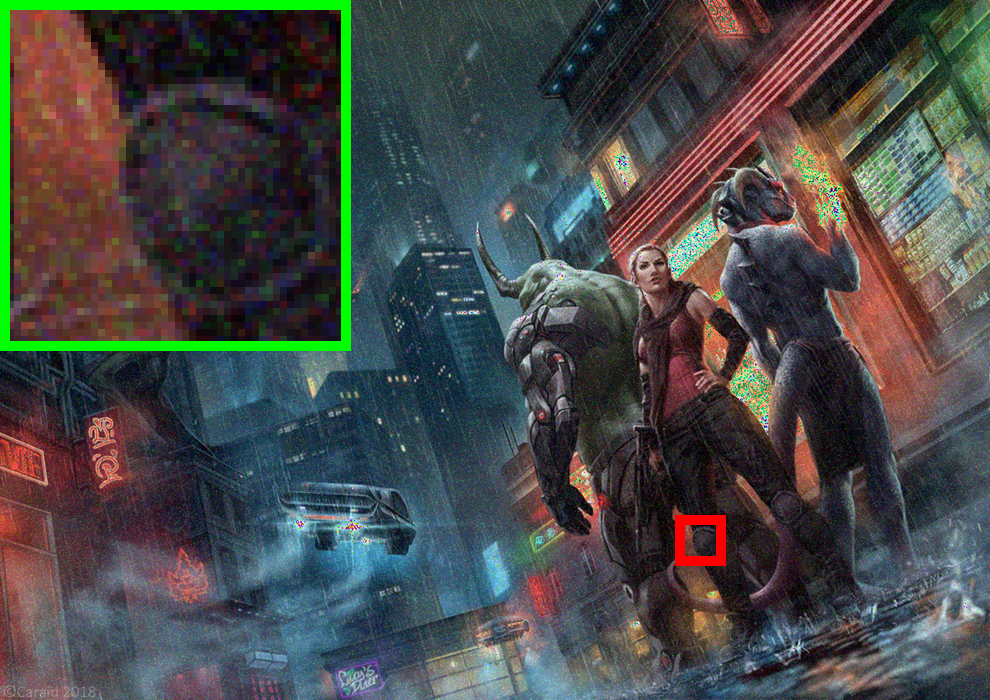
\includegraphics[width=\textwidth]{Figures/2X/Cyberpunk/LR_Cyberpunk_GAUSS_25_comparison.png}
            \caption{LR image with gaussian noise (25$\sigma$)}
        \end{subfigure}
        \hfill
        \begin{subfigure}[b]{0.475\textwidth}  
            \centering 
            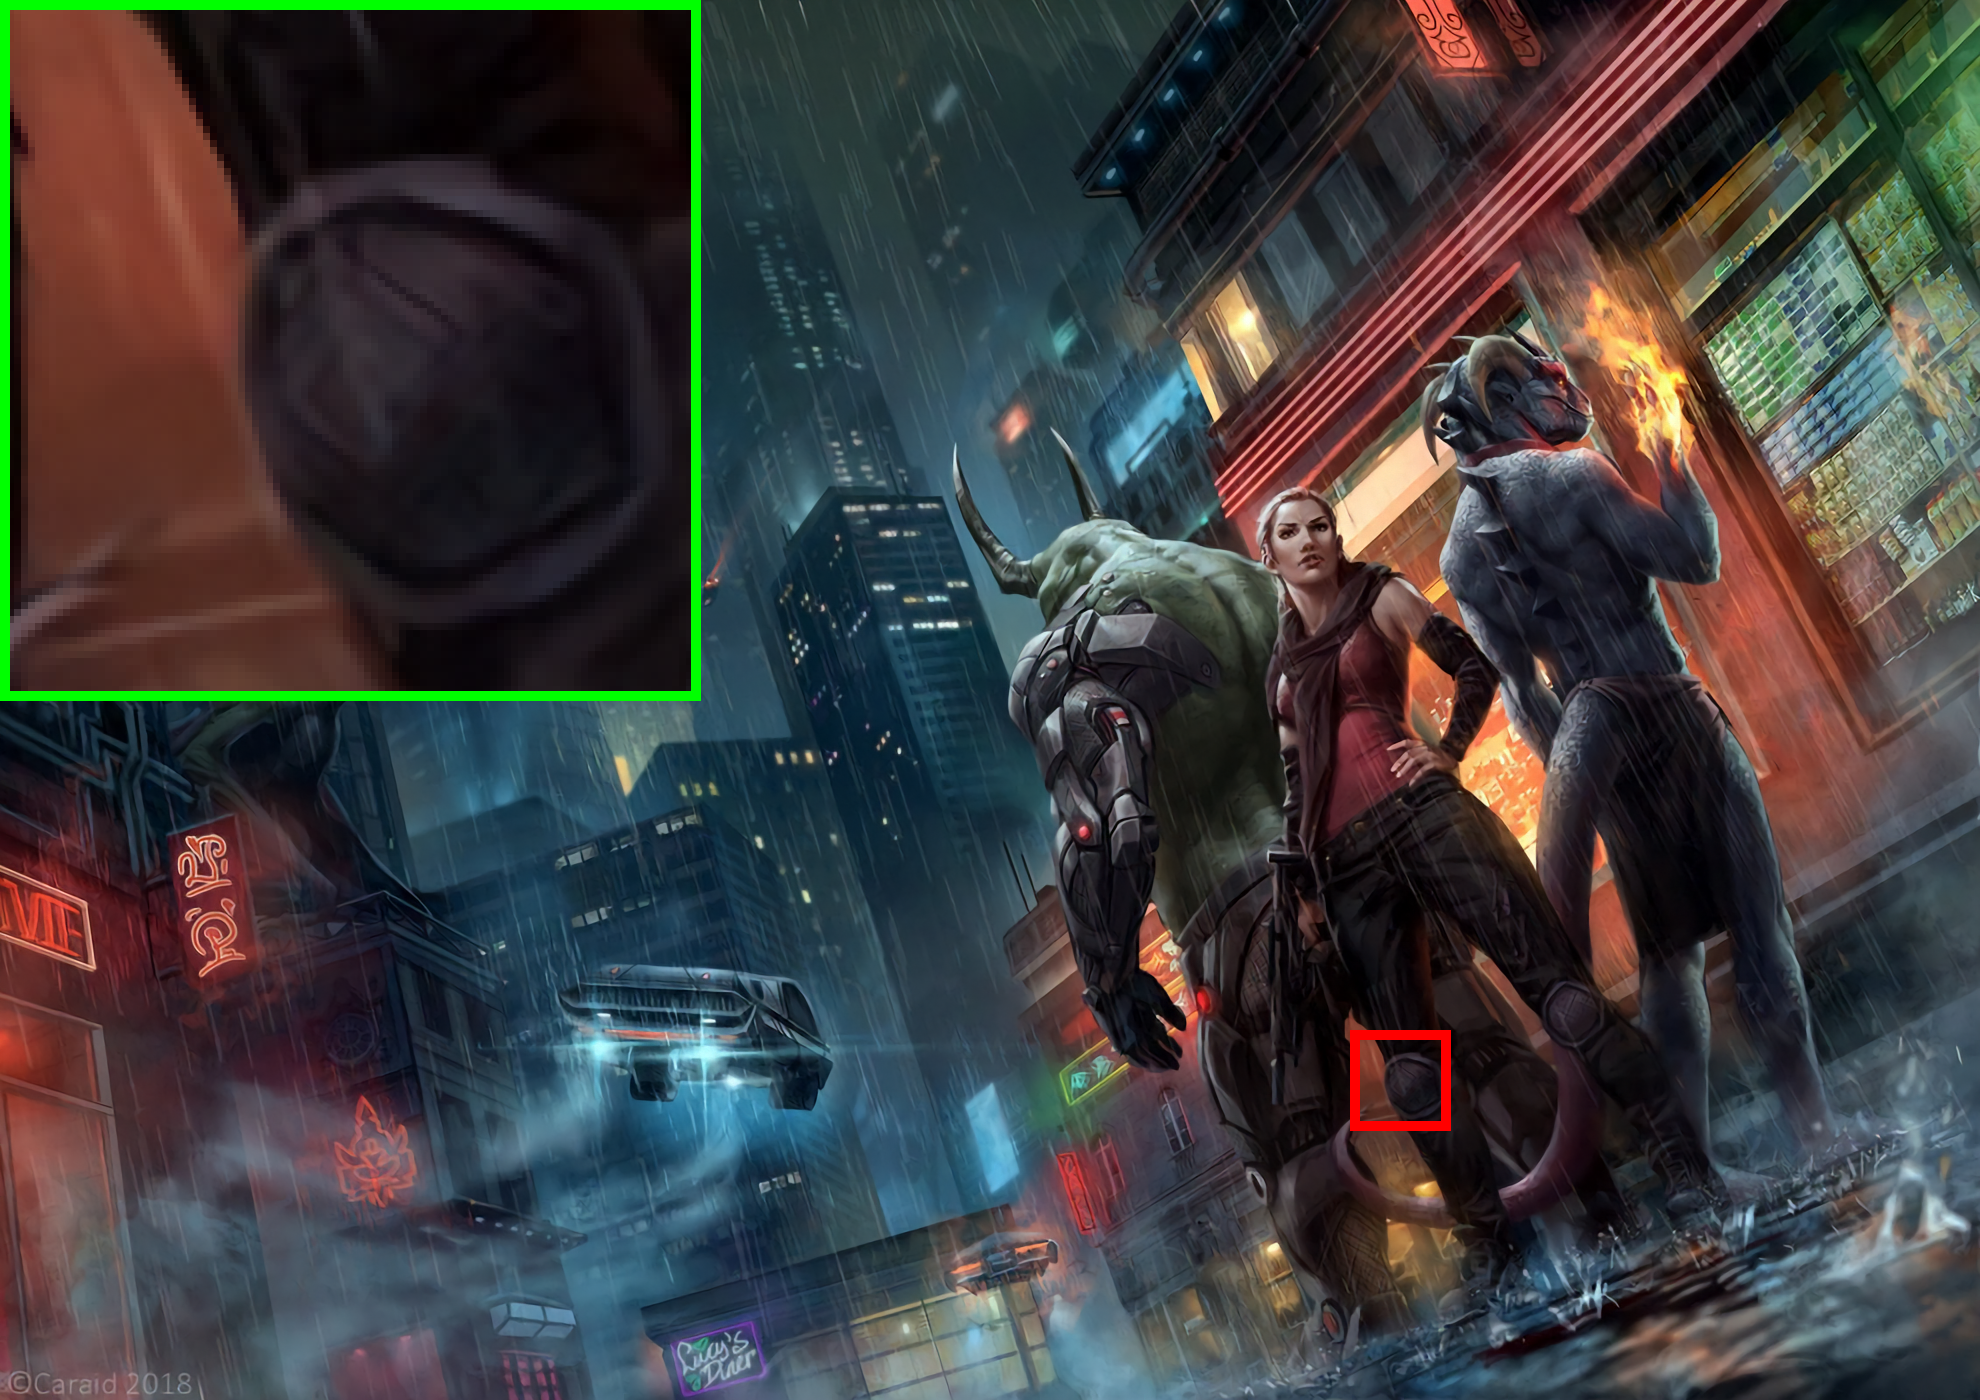
\includegraphics[width=\textwidth]{Figures/2X/Cyberpunk/EDSR_Cyberpunk_GAUSS_25_comparison.png}
            \caption{EDSR result}
        \end{subfigure}
        \vskip\baselineskip
        \begin{subfigure}[b]{0.475\textwidth}   
            \centering 
            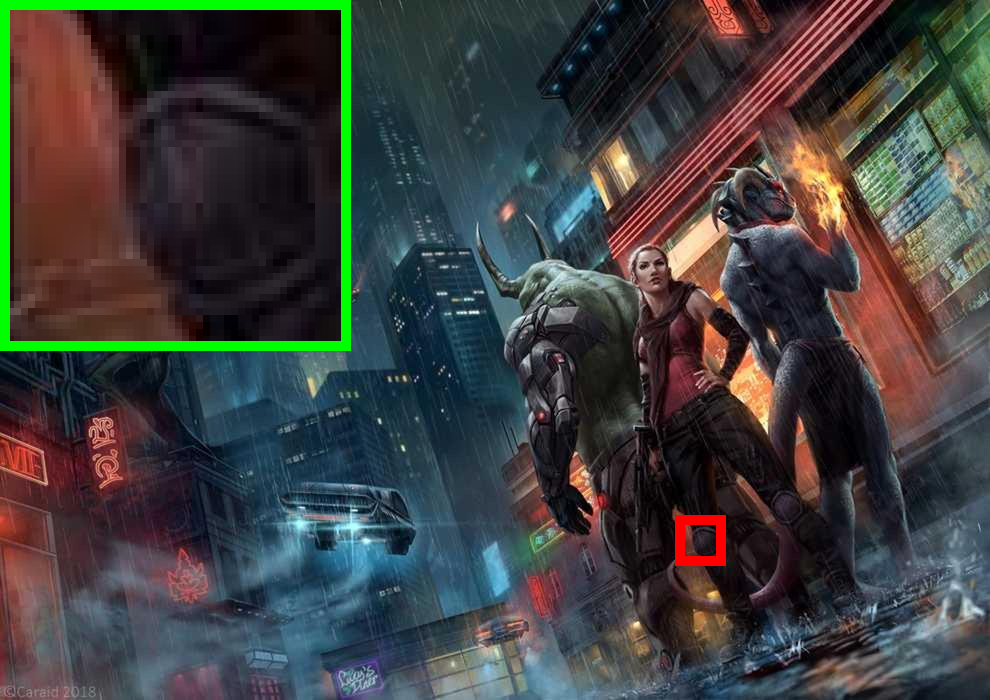
\includegraphics[width=\textwidth]{Figures/2X/Cyberpunk/LR_Cyberpunk_JPEG_50_comparison.png}
            \caption{LR image with JPEG noise (50)}
        \end{subfigure}
        \quad
        \begin{subfigure}[b]{0.475\textwidth}   
            \centering 
            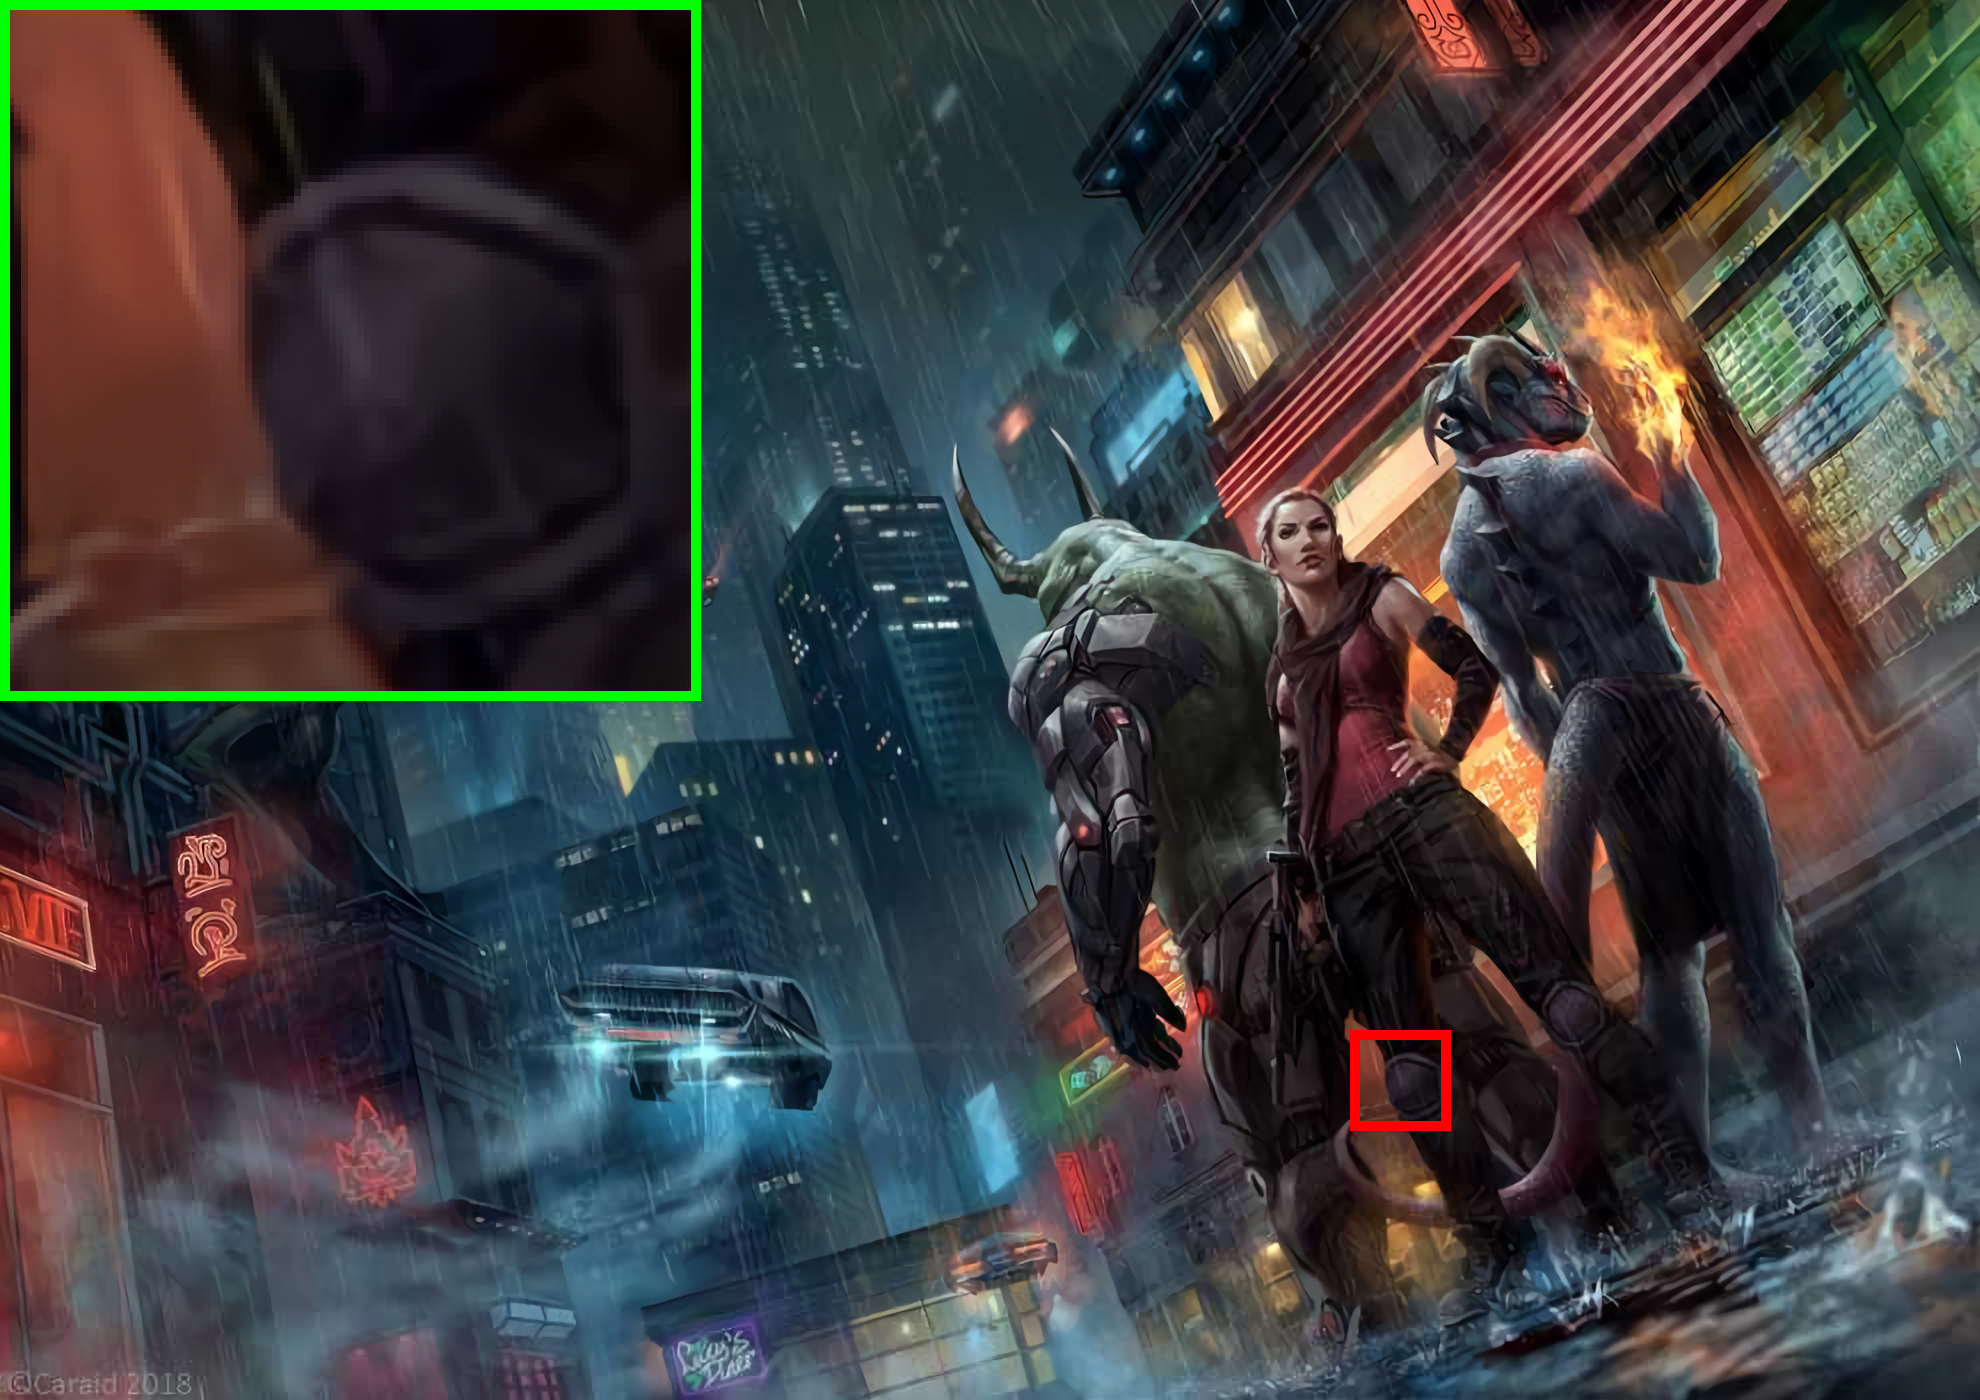
\includegraphics[width=\textwidth]{Figures/2X/Cyberpunk/EDSR_Cyberpunk_JPEG_50_comparison.png}
            \caption{EDSR result}
        \end{subfigure}
        \caption{trained denoising capabilities}
\end{figure}


\begin{figure*}
        \centering
        \begin{subfigure}[b]{0.475\textwidth}
            \centering
            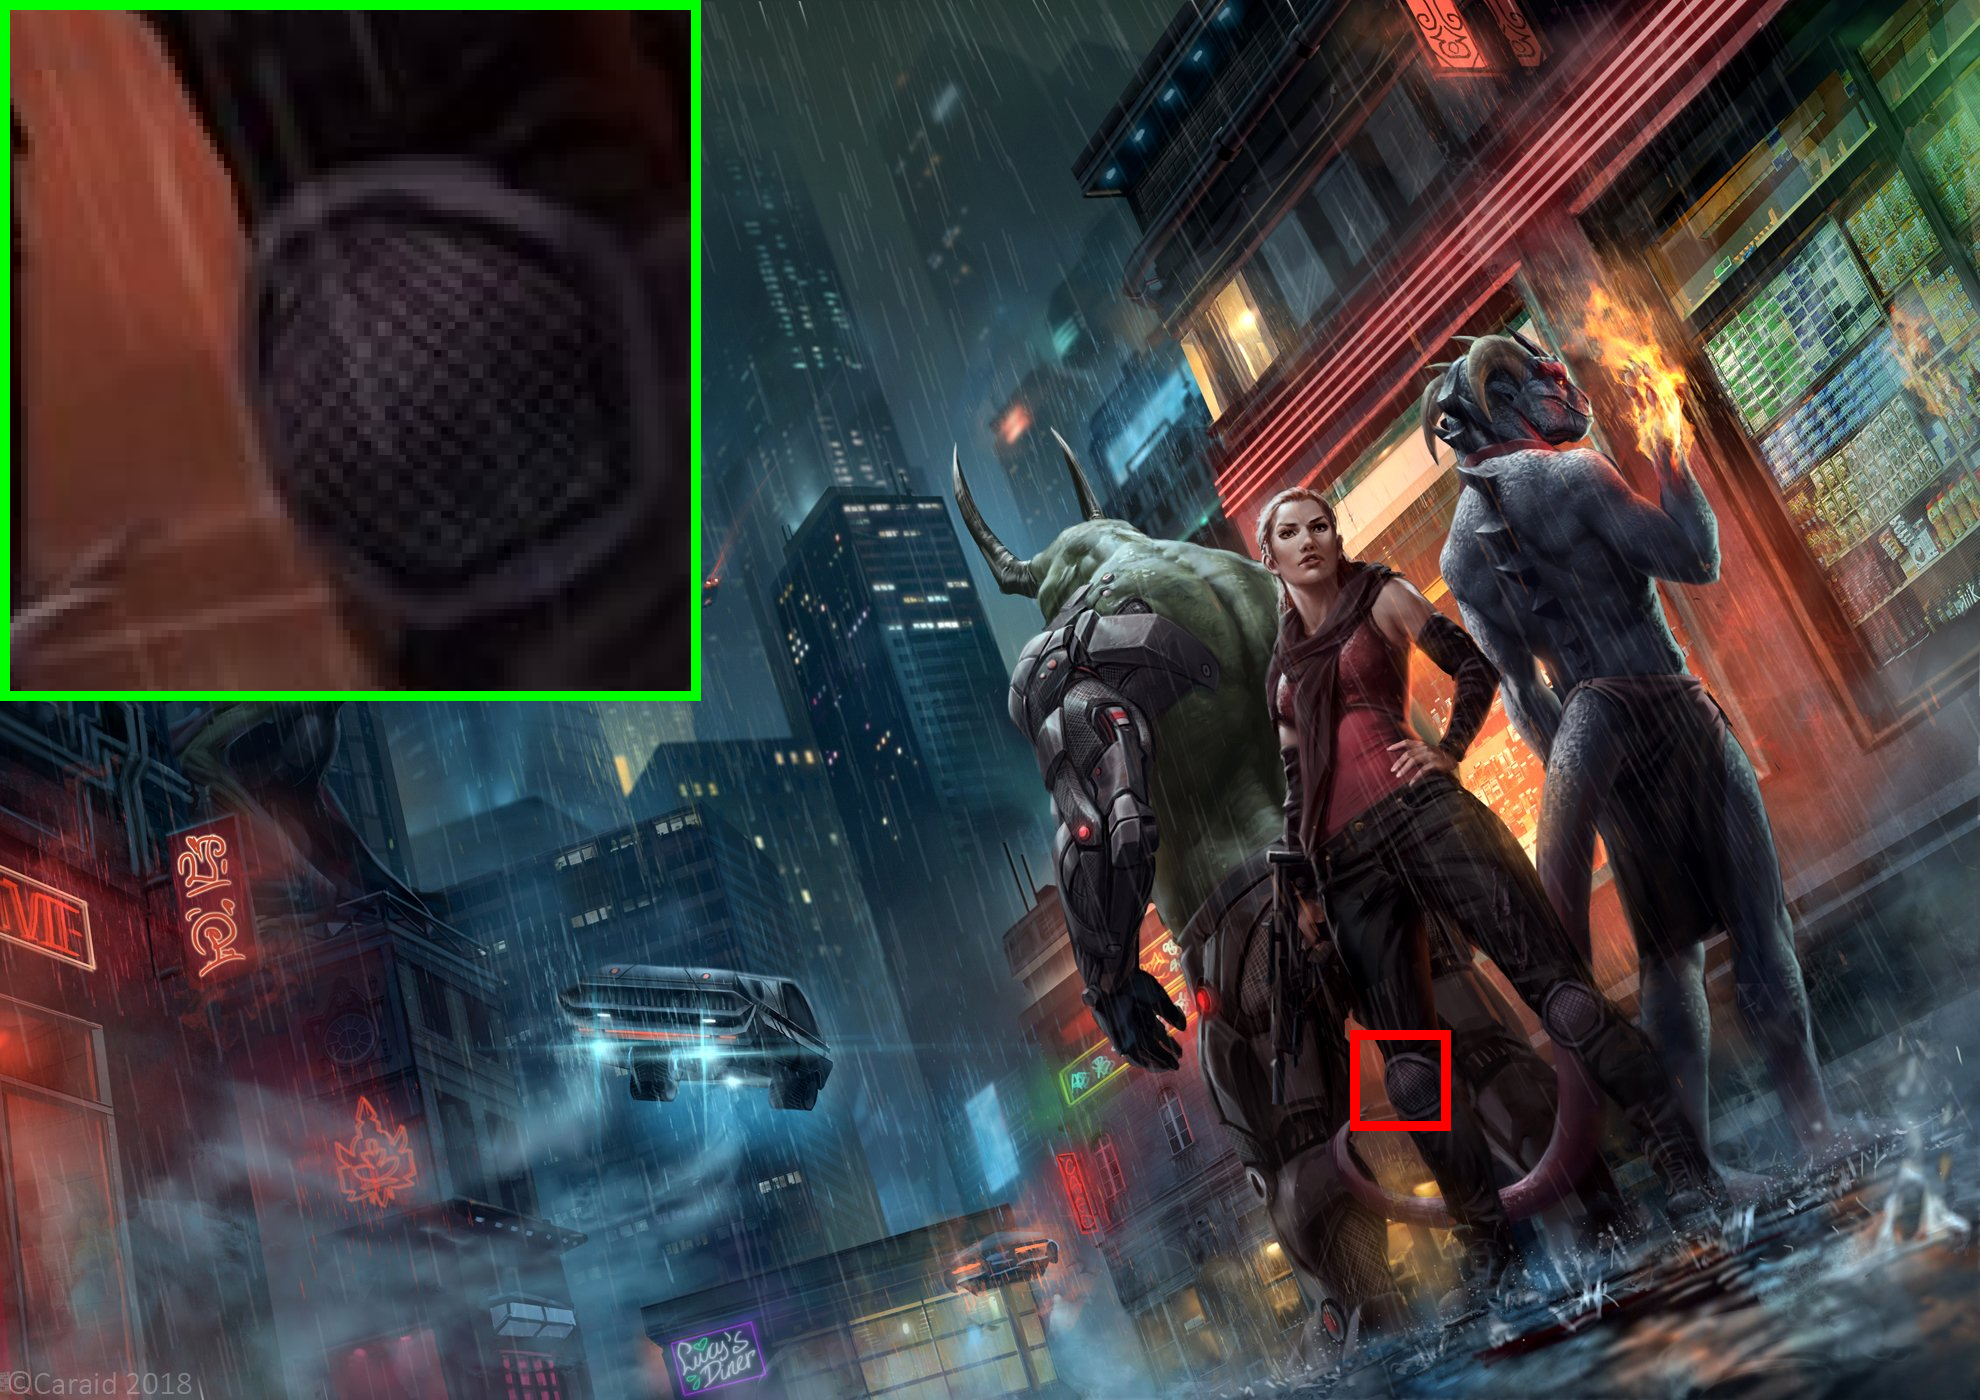
\includegraphics[width=\textwidth]{Figures/2X/Cyberpunk/Cyberpunk_HR.png}
            \caption{High Resolution}
        \end{subfigure}
        \vskip\baselineskip
        \begin{subfigure}[b]{0.475\textwidth}
            \centering
            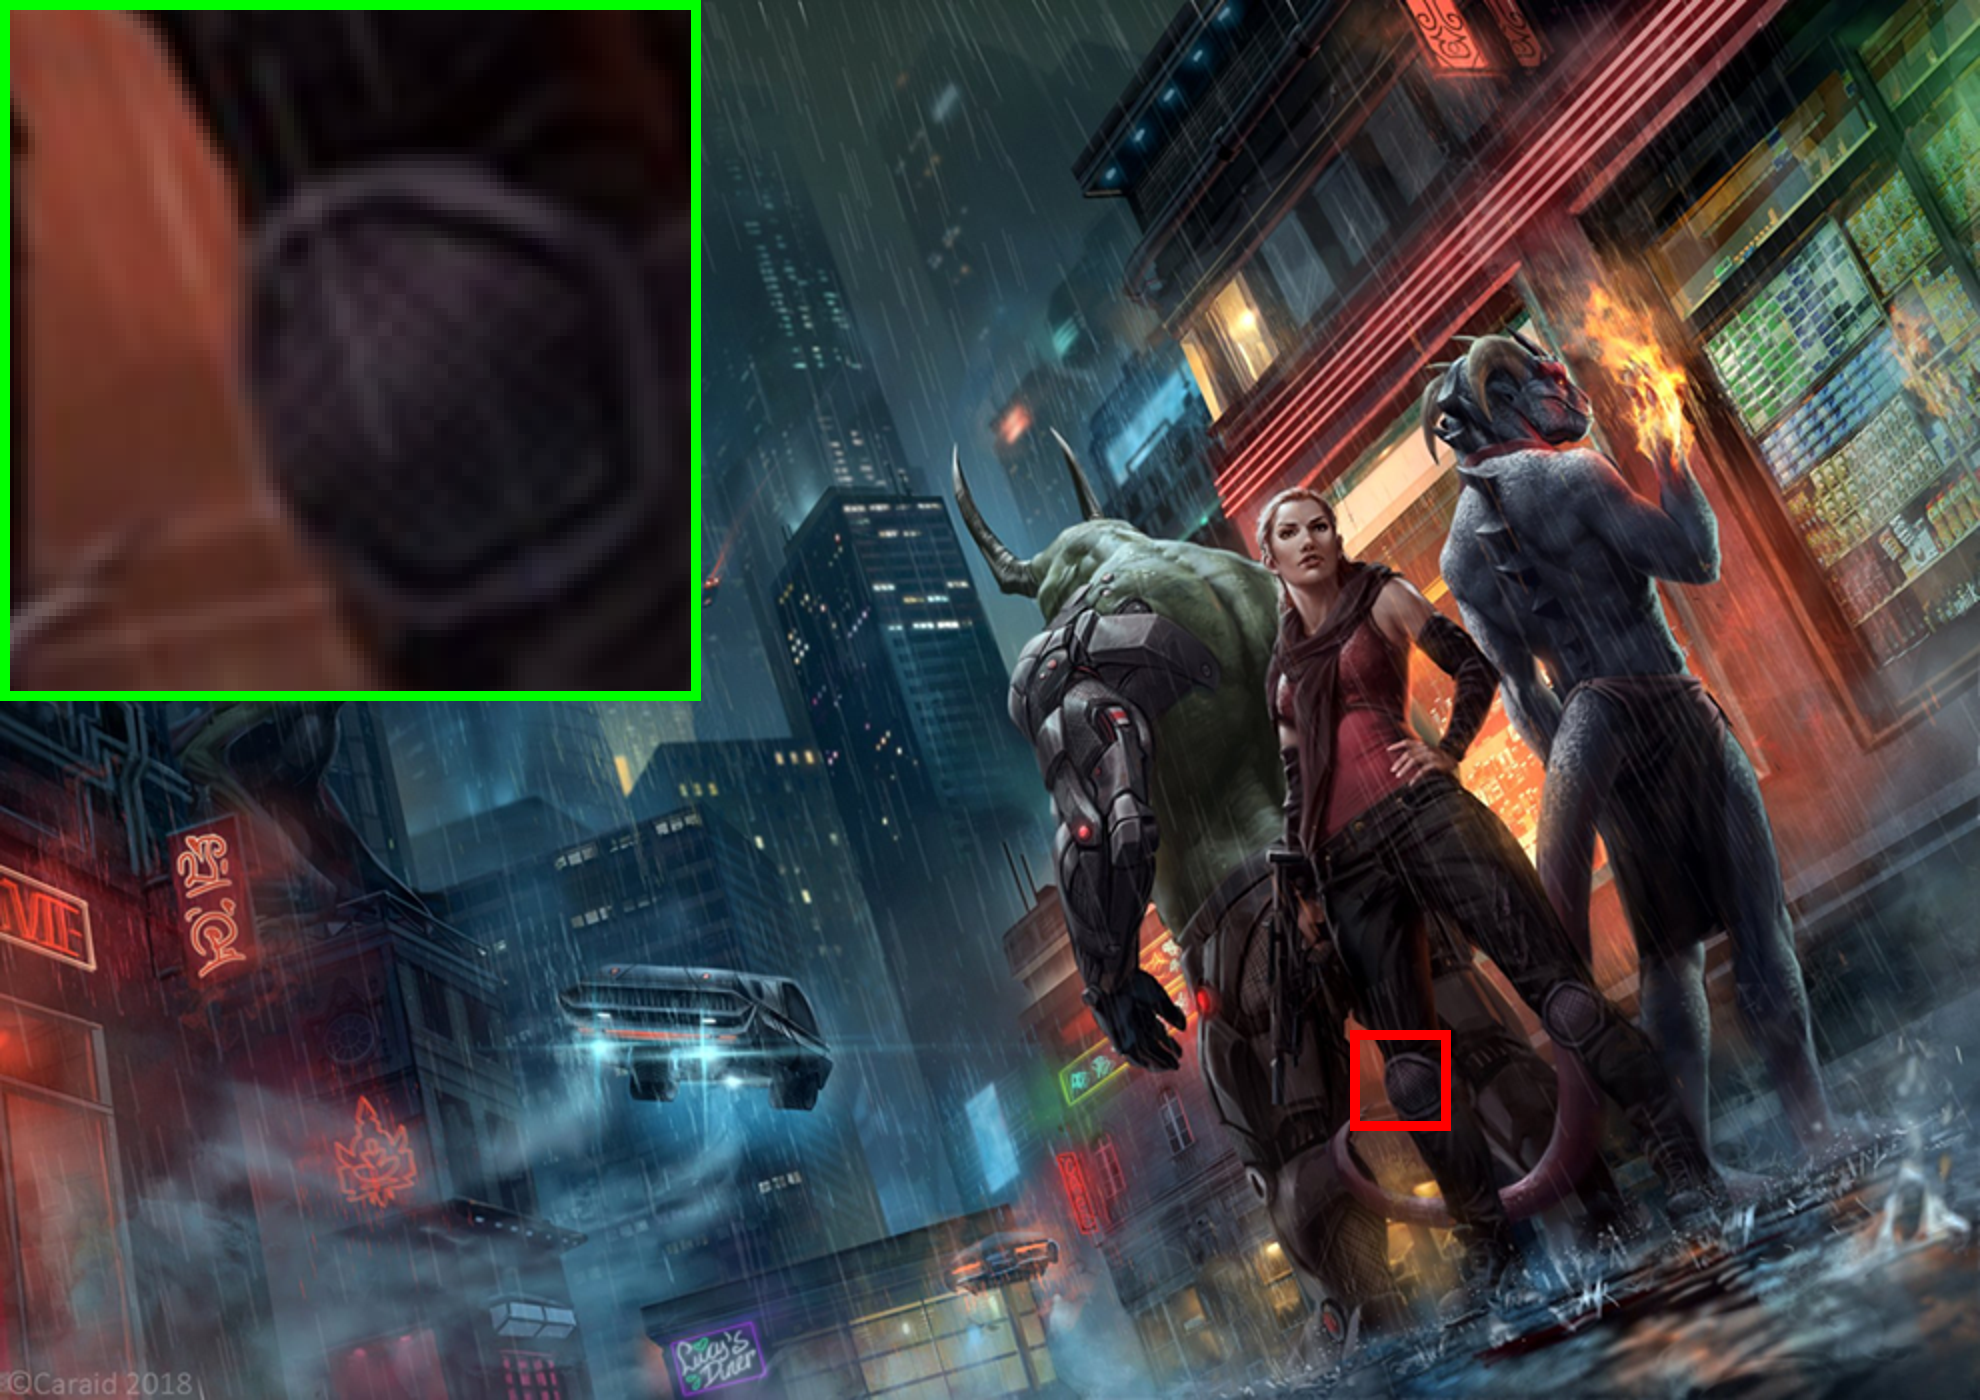
\includegraphics[width=\textwidth]{Figures/2X/Cyberpunk/Bicubic_Cyberpunk_GAUSS_0_comparison.png}
            \caption{Bicubic}
        \end{subfigure}
        \hfill
        \begin{subfigure}[b]{0.475\textwidth}  
            \centering 
            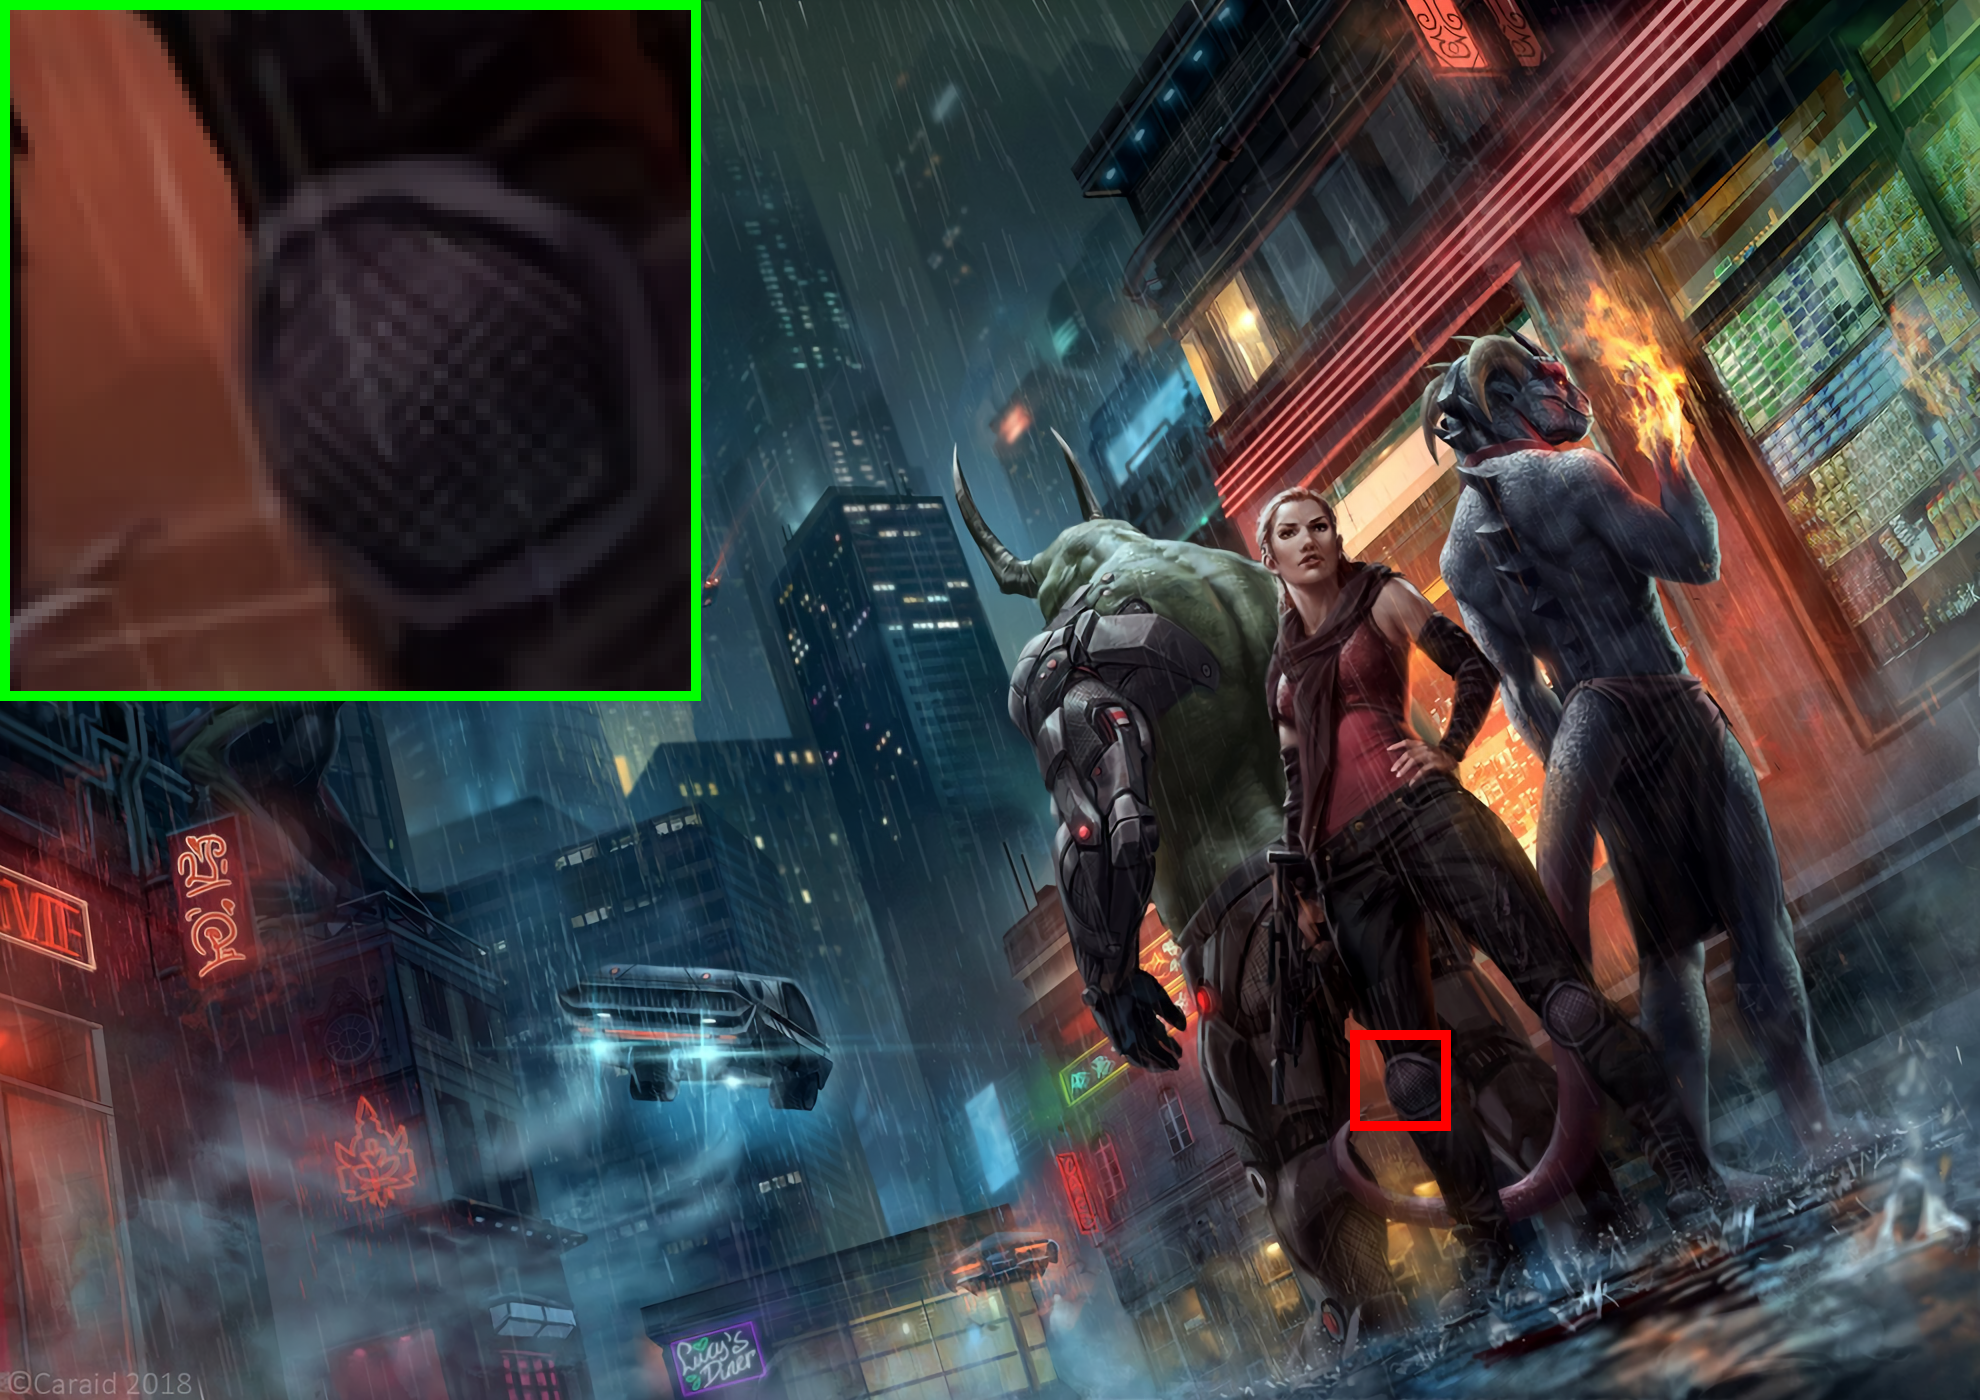
\includegraphics[width=\textwidth]{Figures/2X/Cyberpunk/EDSR_Cyberpunk_GAUSS_0_comparison.png}
            \caption{EDSR}     
        \end{subfigure}
        \vskip\baselineskip
        \begin{subfigure}[b]{0.475\textwidth}   
            \centering 
            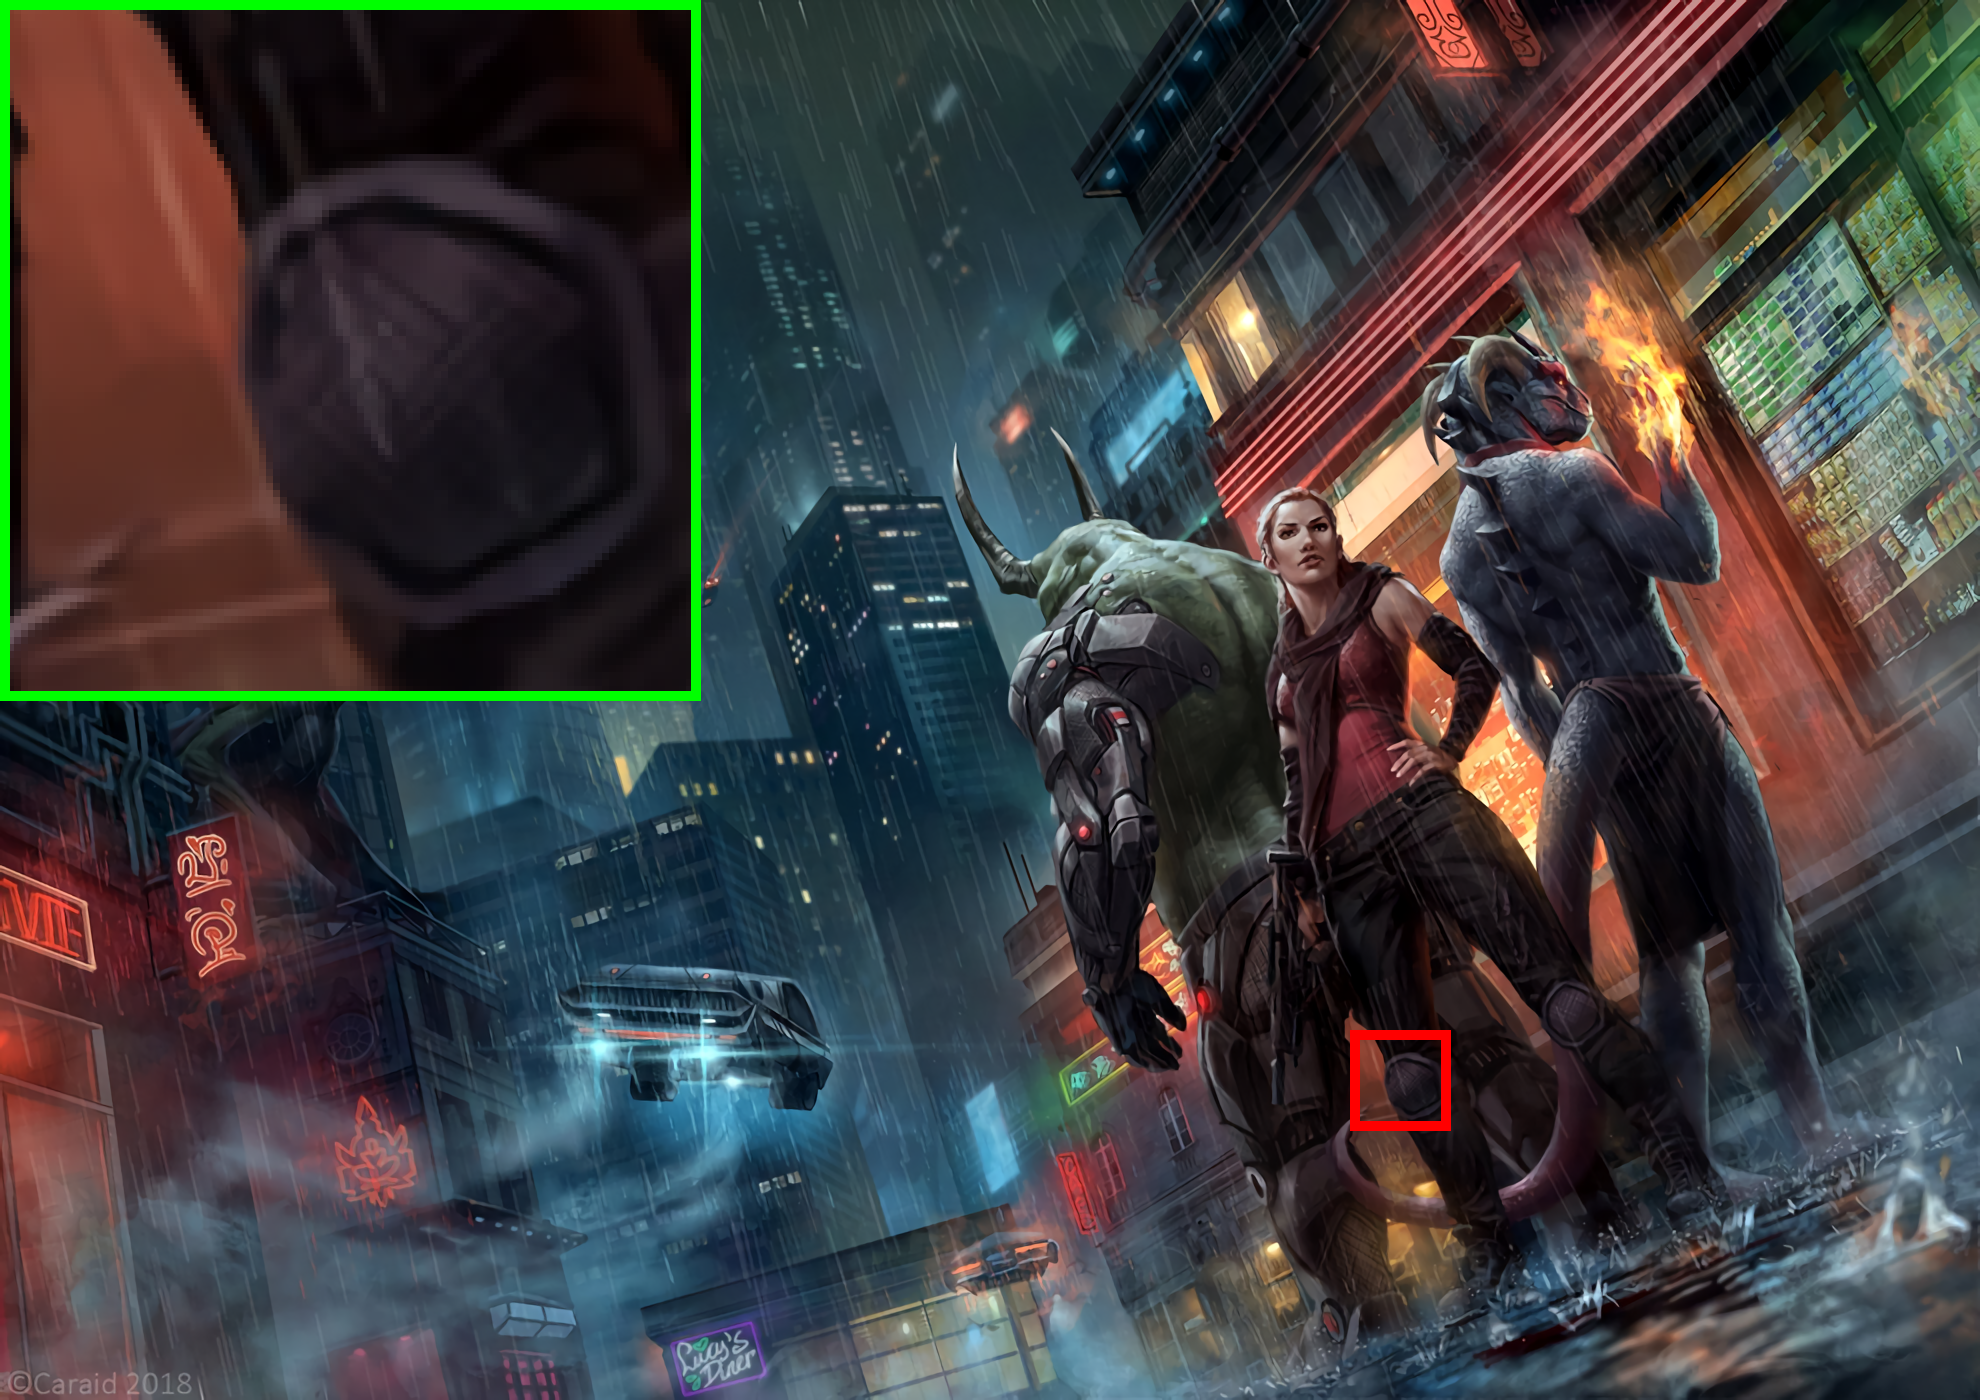
\includegraphics[width=\textwidth]{Figures/2X/Cyberpunk/Waifu2X_0_Cyberpunk_GAUSS_0_comparison.png}
            \caption{Waifu2x (level 0)}  
        \end{subfigure}
        \quad
        \begin{subfigure}[b]{0.475\textwidth}   
            \centering 
            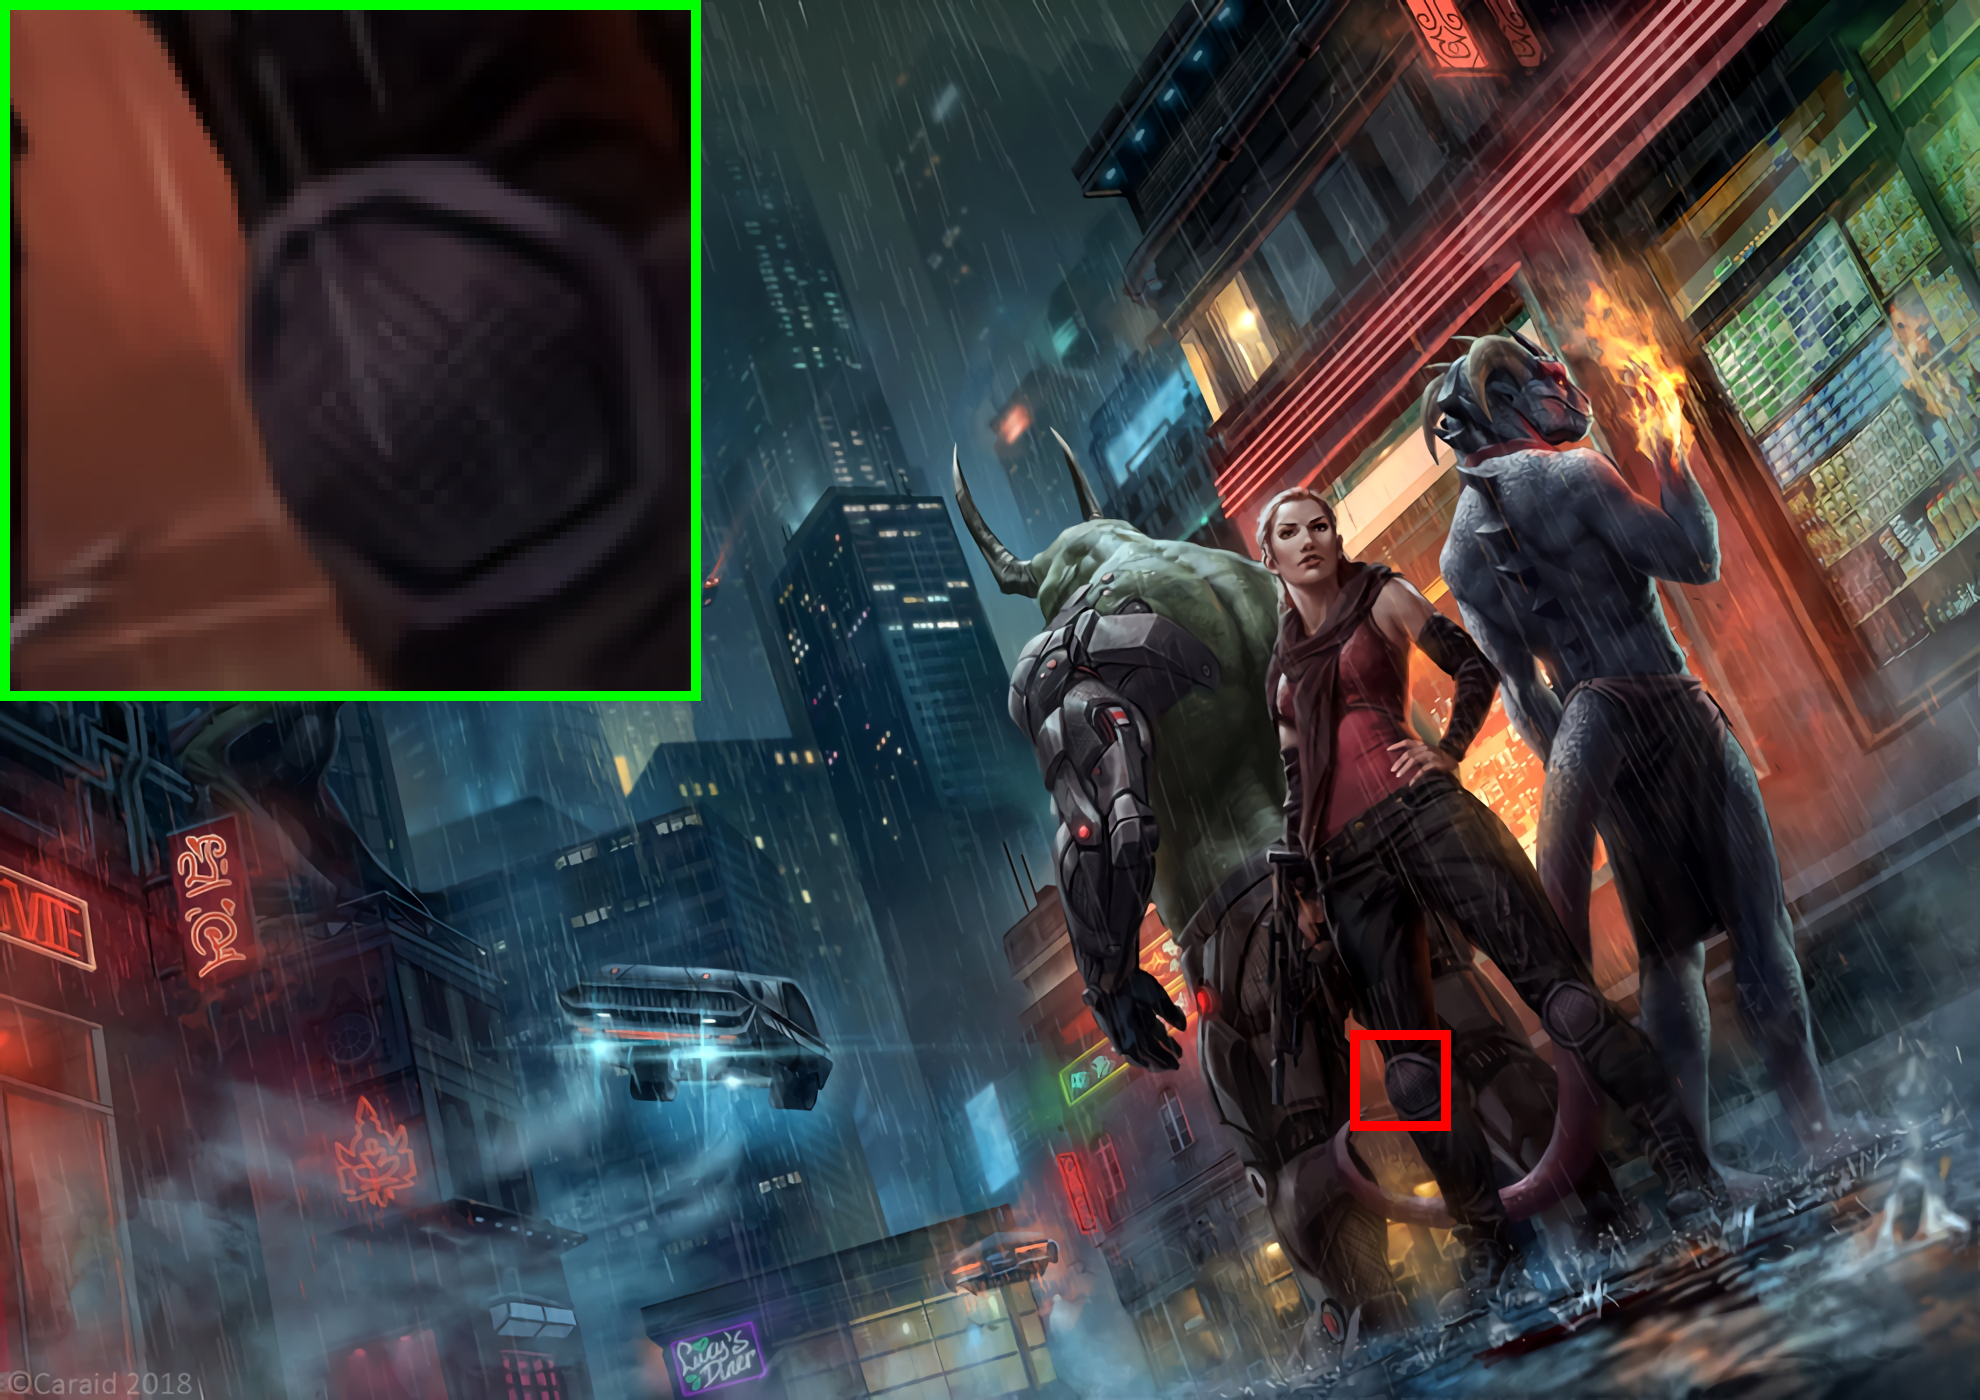
\includegraphics[width=\textwidth]{Figures/2X/Cyberpunk/Waifu2X_1_Cyberpunk_GAUSS_0_comparison.png}
            \caption{Waifu2x (level 1)}  
        \end{subfigure}
        \vskip\baselineskip
        \begin{subfigure}[b]{0.475\textwidth}   
            \centering 
            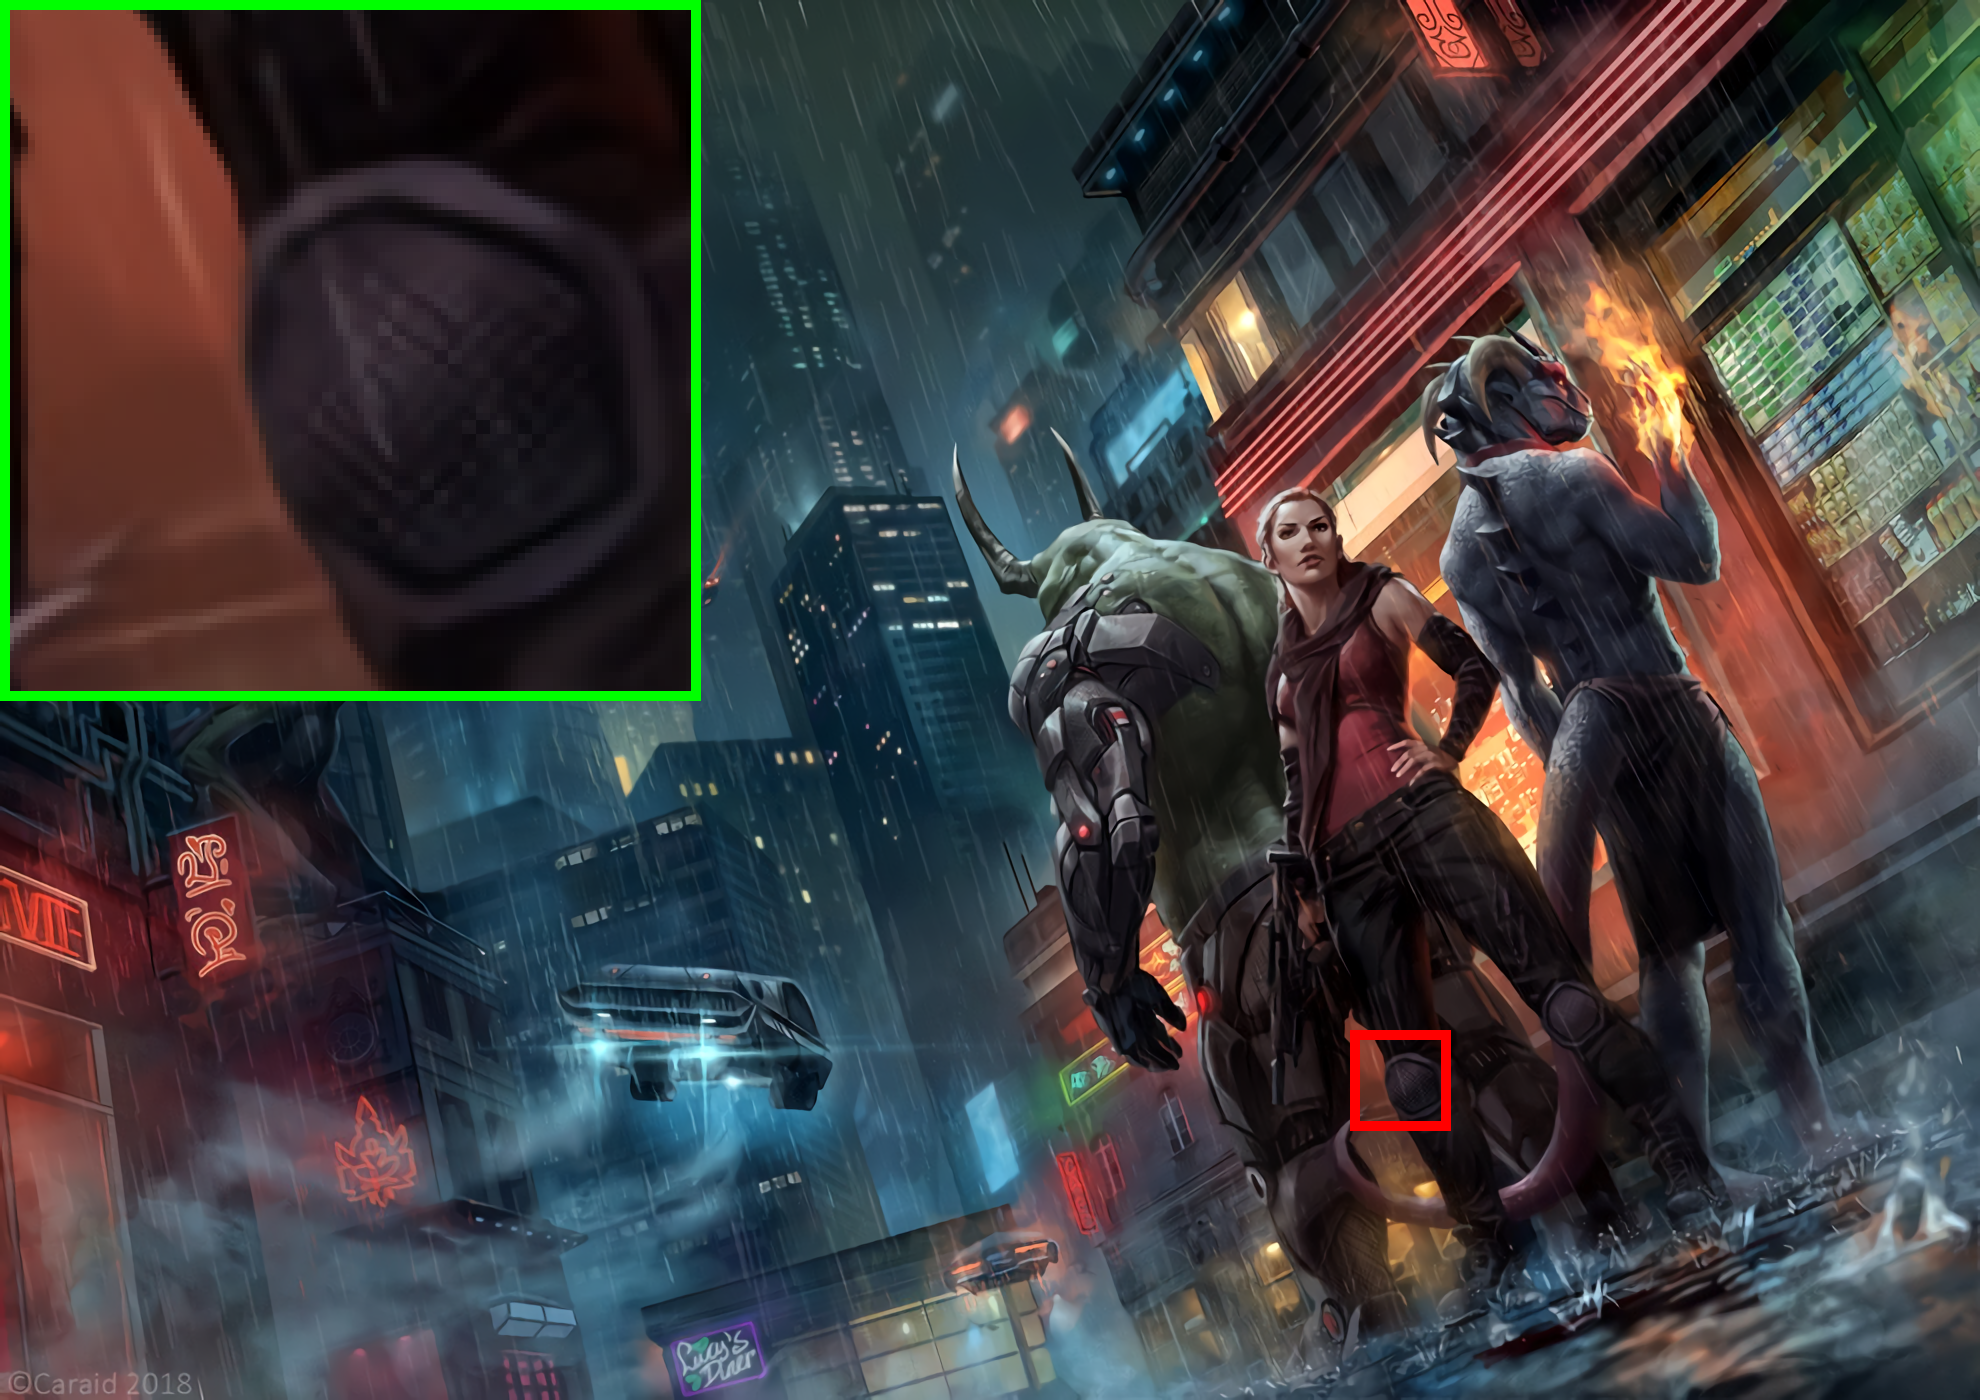
\includegraphics[width=\textwidth]{Figures/2X/Cyberpunk/Waifu2X_2_Cyberpunk_GAUSS_0_comparison.png}
            \caption{Waifu2x (level 2)}  
        \end{subfigure}
        \quad
        \begin{subfigure}[b]{0.475\textwidth}   
            \centering 
            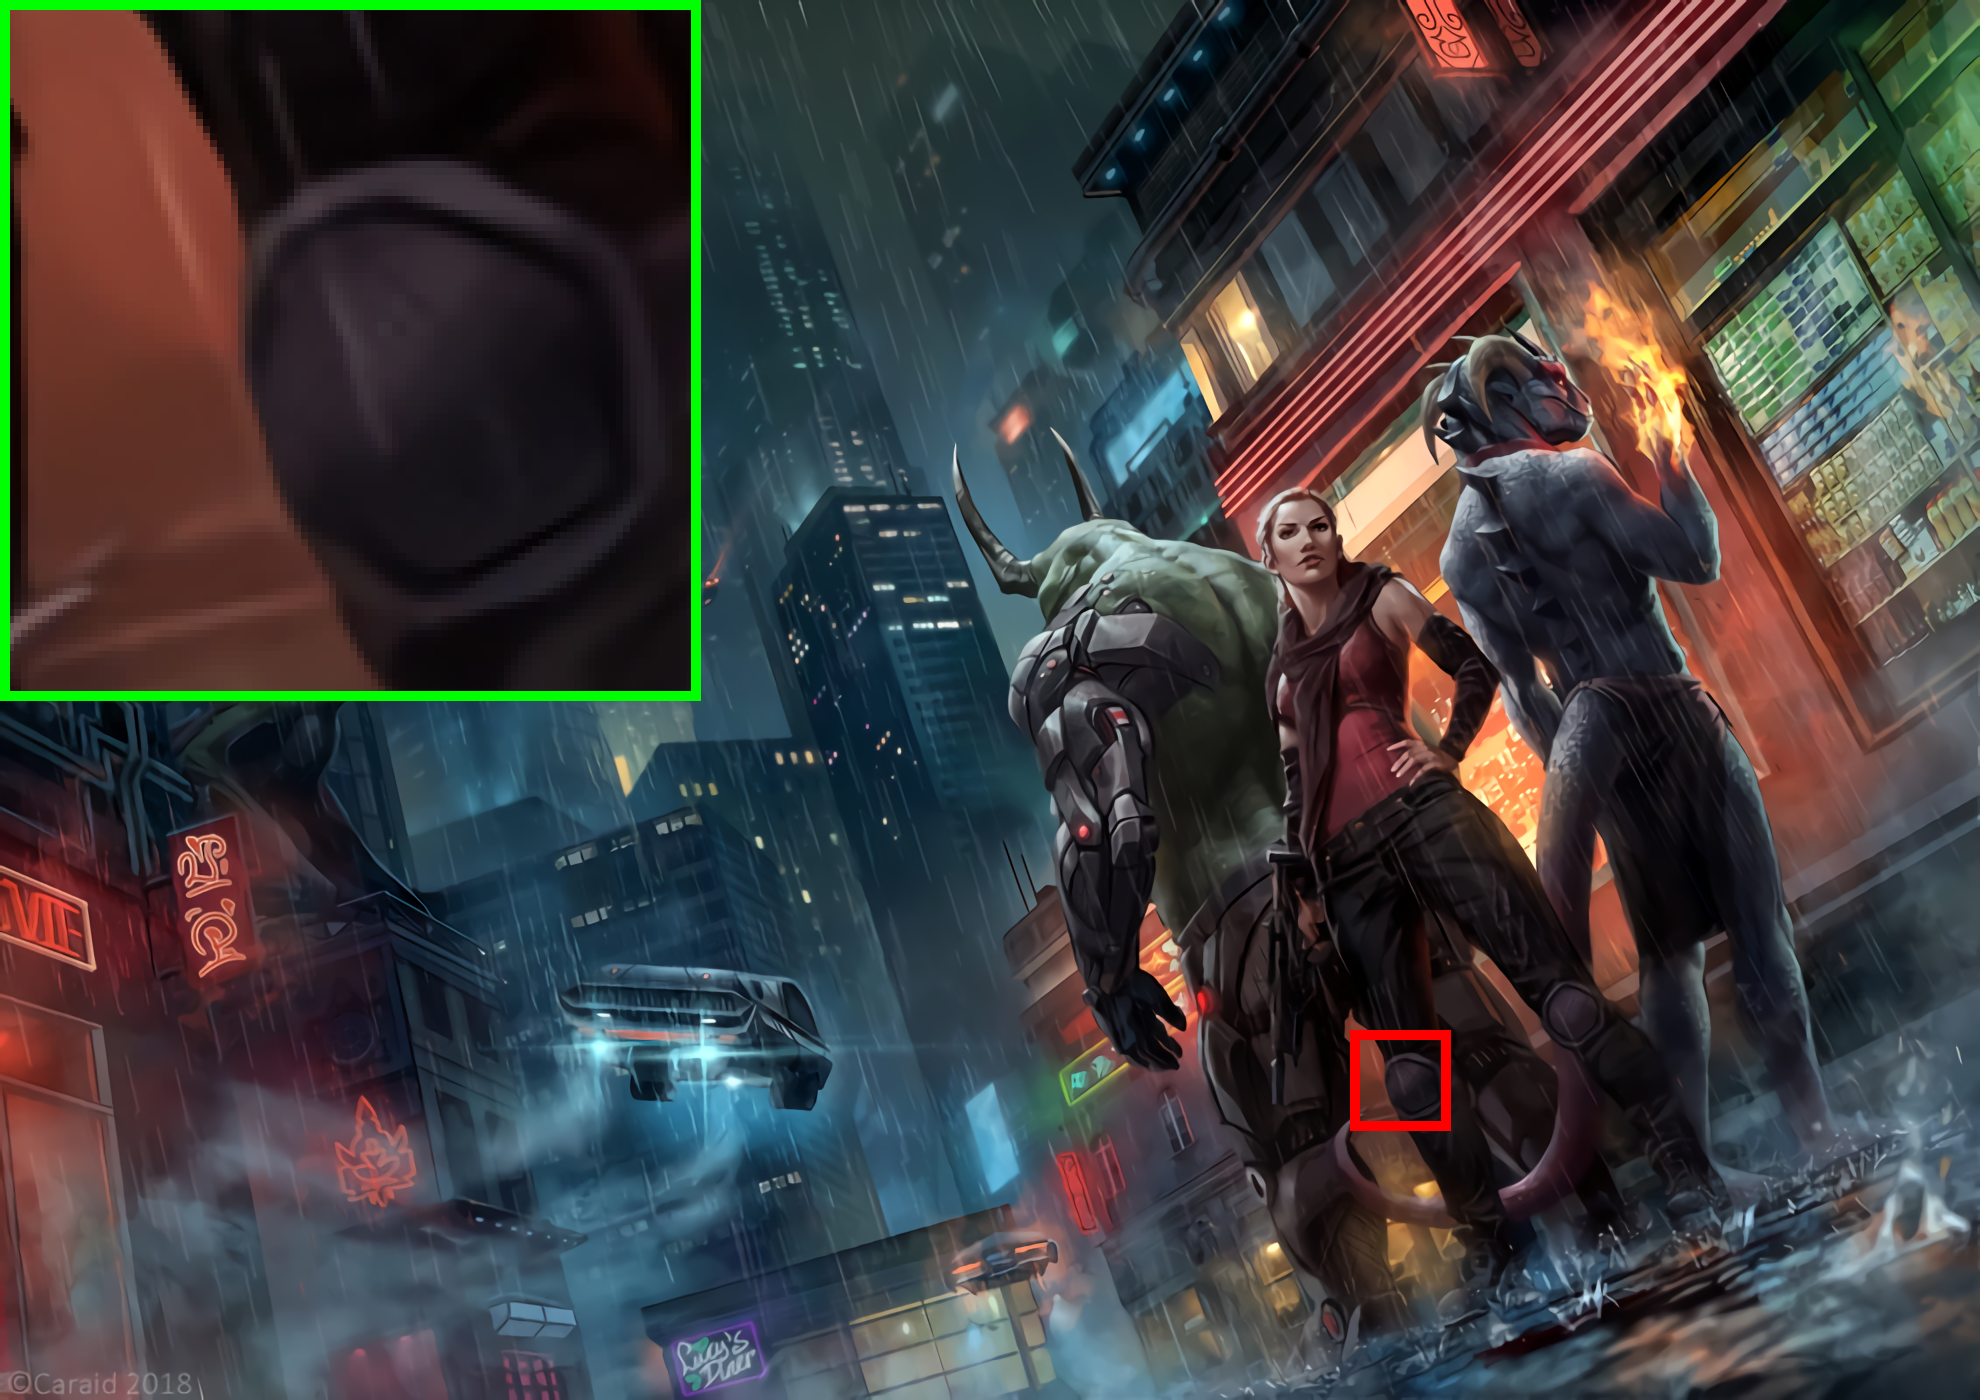
\includegraphics[width=\textwidth]{Figures/2X/Cyberpunk/Waifu2X_3_Cyberpunk_GAUSS_0_comparison.png}
            \caption{Waifu2x (level 3)}  
        \end{subfigure}
        \caption{Results of Waifu2x and my trained model on a clean version (GAUSS\_0) of one of the images}  
                \label{Cyberpunk_fig}
    \end{figure*}
    
    \begin{figure*}
        \centering
        \begin{subfigure}[b]{0.75\textwidth}
            \centering
            \includegraphics[width=\textwidth]{Figures/2X/Cyberpunk/be15968553390b112e723e8773910e11.png}
            \caption{High Resolution}
        \end{subfigure}
        \vskip\baselineskip
        \begin{subfigure}[b]{0.475\textwidth}
            \centering
            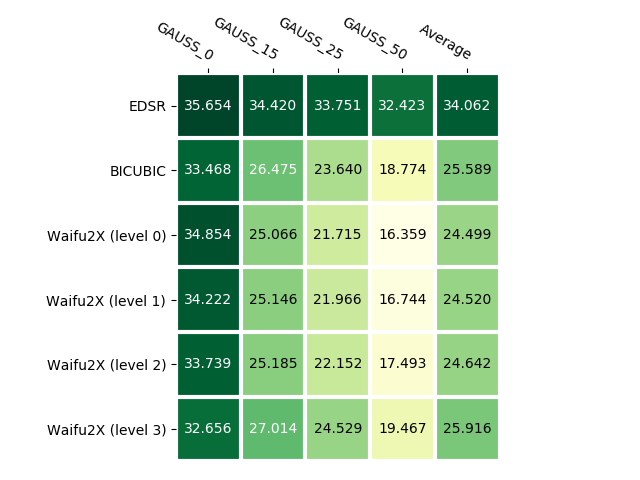
\includegraphics[width=\textwidth]{Figures/2X/Cyberpunk/PSNR_GAUSS_Cyberpunk.png}
            \caption{PSNR results with gaussian noise}
        \end{subfigure}
        \hfill
        \begin{subfigure}[b]{0.475\textwidth}  
            \centering 
            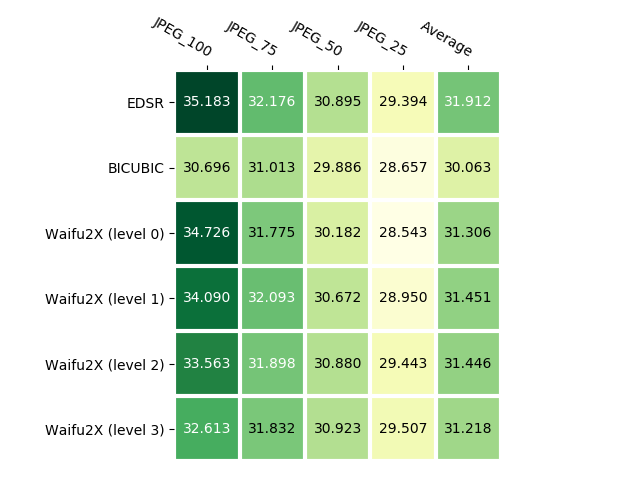
\includegraphics[width=\textwidth]{Figures/2X/Cyberpunk/PSNR_JPEG_Cyberpunk.png}
            \caption{PSNR results with JPEG noise}
        \end{subfigure}
        \vskip\baselineskip
        \begin{subfigure}[b]{0.475\textwidth}   
            \centering 
            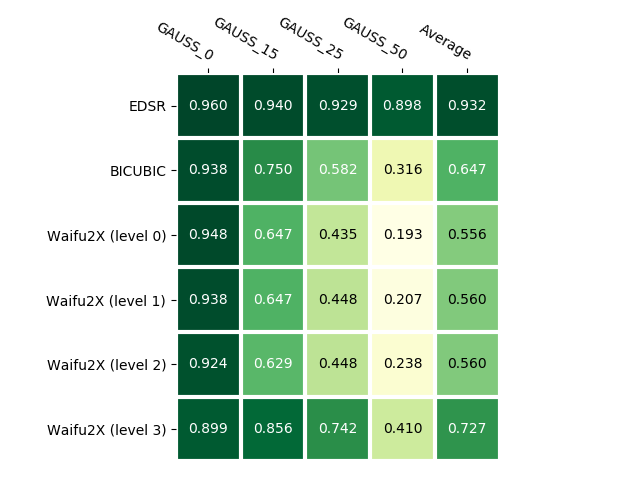
\includegraphics[width=\textwidth]{Figures/2X/Cyberpunk/SSIM_GAUSS_Cyberpunk.png}
            \caption{SSIM results with gaussian noise}
        \end{subfigure}
        \quad
        \begin{subfigure}[b]{0.475\textwidth}   
            \centering 
            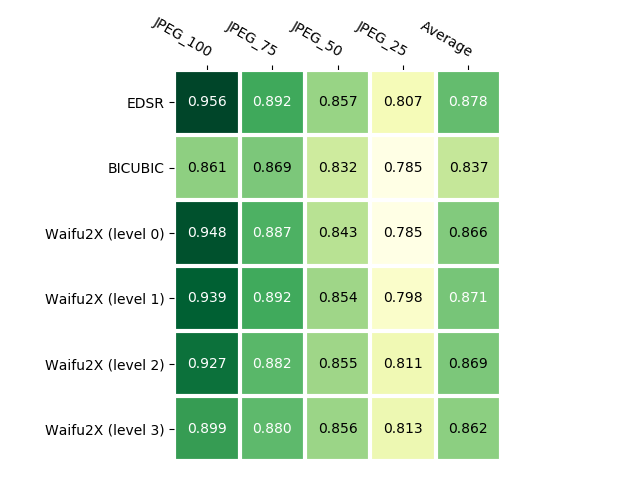
\includegraphics[width=\textwidth]{Figures/2X/Cyberpunk/SSIM_JPEG_Cyberpunk.png}
            \caption{SSIM results with JPEG noise}
        \end{subfigure}
        \caption{PSNR and SSIM results on the shown image}
    \end{figure*}
    
    \begin{figure*}
        \centering
        \begin{subfigure}[b]{0.75\textwidth}
            \centering
            \includegraphics[width=\textwidth]{Figures/2X/Tiger/image.png}
            \caption{High Resolution}
        \end{subfigure}
        \vskip\baselineskip
        \begin{subfigure}[b]{0.475\textwidth}
            \centering
            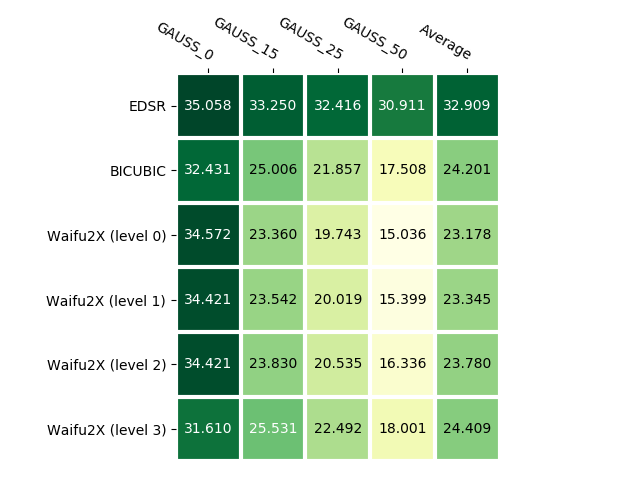
\includegraphics[width=\textwidth]{Figures/2X/Tiger/PSNR_GAUSS.png}
            \caption{PSNR results with gaussian noise}
        \end{subfigure}
        \hfill
        \begin{subfigure}[b]{0.475\textwidth}  
            \centering 
            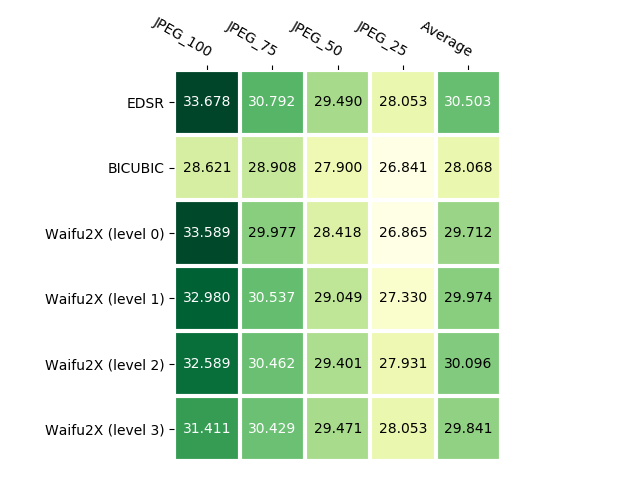
\includegraphics[width=\textwidth]{Figures/2X/Tiger/PSNR_JPEG.png}
            \caption{PSNR results with JPEG noise}
        \end{subfigure}
        \vskip\baselineskip
        \begin{subfigure}[b]{0.475\textwidth}   
            \centering 
            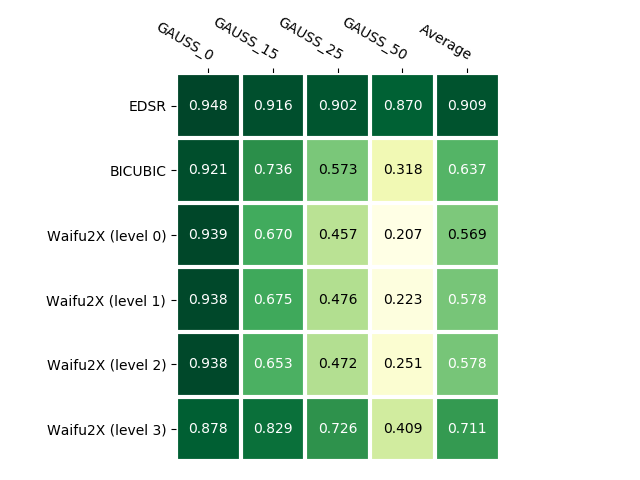
\includegraphics[width=\textwidth]{Figures/2X/Tiger/SSIM_GAUSS.png}
            \caption{SSIM results with gaussian noise}
        \end{subfigure}
        \quad
        \begin{subfigure}[b]{0.475\textwidth}   
            \centering 
            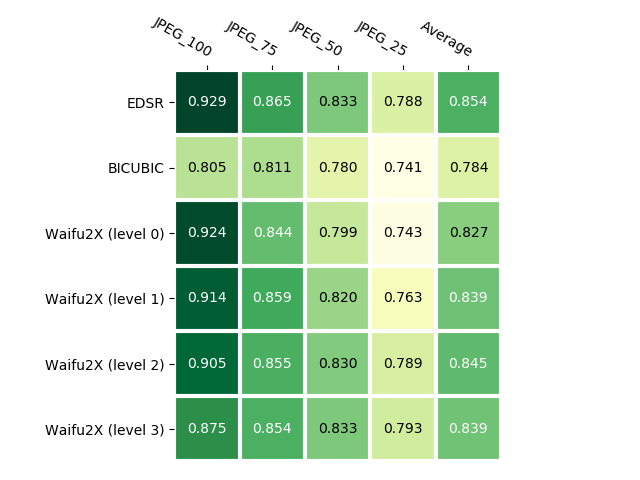
\includegraphics[width=\textwidth]{Figures/2X/Tiger/SSIM_JPEG.png}
            \caption{SSIM results with JPEG noise}
        \end{subfigure}
        \caption{PSNR and SSIM results on the shown image}
    \end{figure*}
    
        \begin{figure*}
        \centering
        \begin{subfigure}[b]{0.75\textwidth}
            \centering
            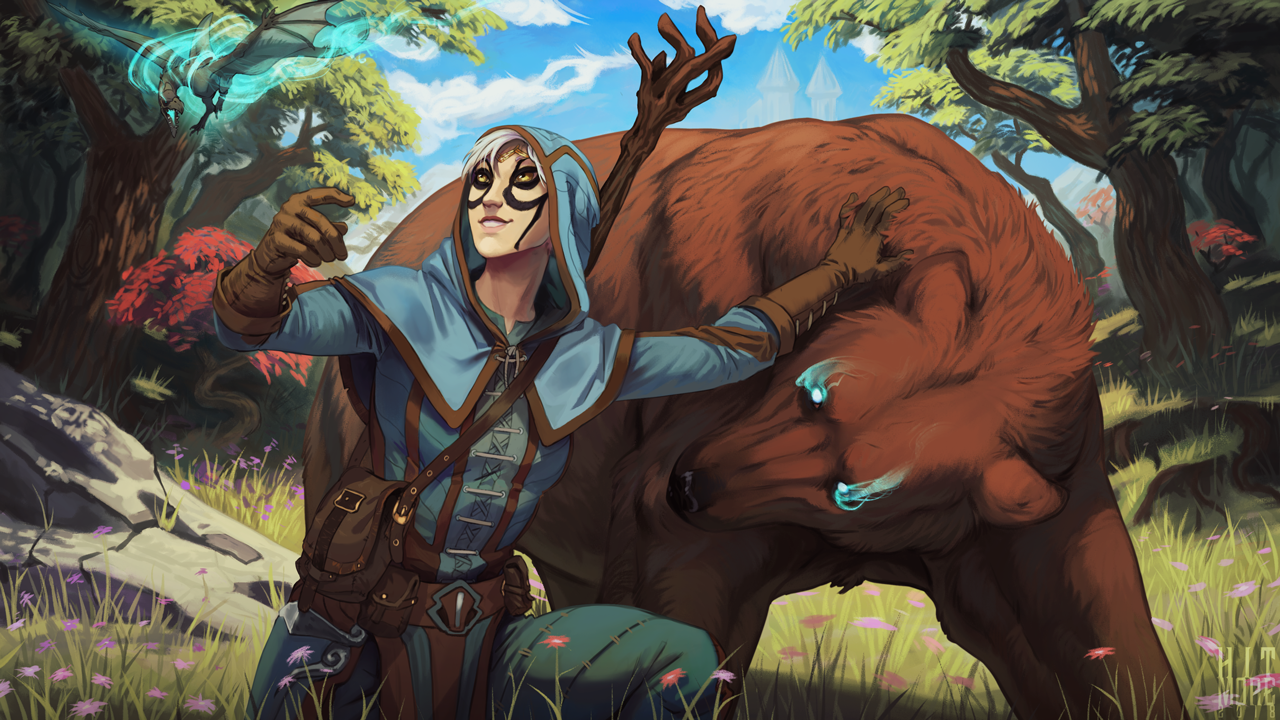
\includegraphics[width=\textwidth]{Figures/2X/Bear/image.png}
            \caption{High Resolution}
        \end{subfigure}
        \vskip\baselineskip
        \begin{subfigure}[b]{0.475\textwidth}
            \centering
            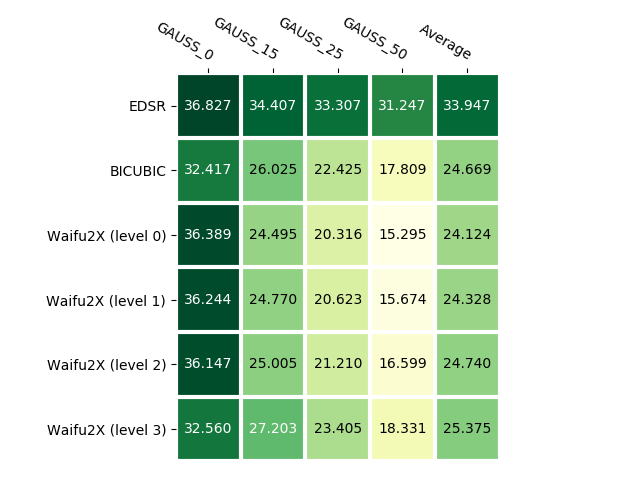
\includegraphics[width=\textwidth]{Figures/2X/Bear/PSNR_GAUSS.png}
            \caption{PSNR results with gaussian noise}
        \end{subfigure}
        \hfill
        \begin{subfigure}[b]{0.475\textwidth}  
            \centering 
            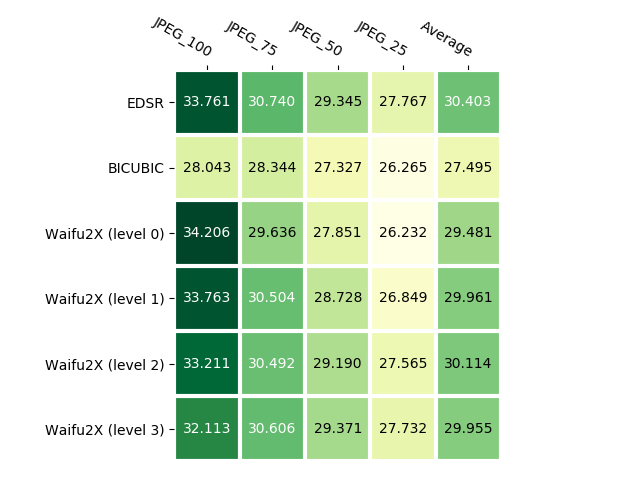
\includegraphics[width=\textwidth]{Figures/2X/Bear/PSNR_JPEG.png}
            \caption{PSNR results with JPEG noise}
        \end{subfigure}
        \vskip\baselineskip
        \begin{subfigure}[b]{0.475\textwidth}   
            \centering 
            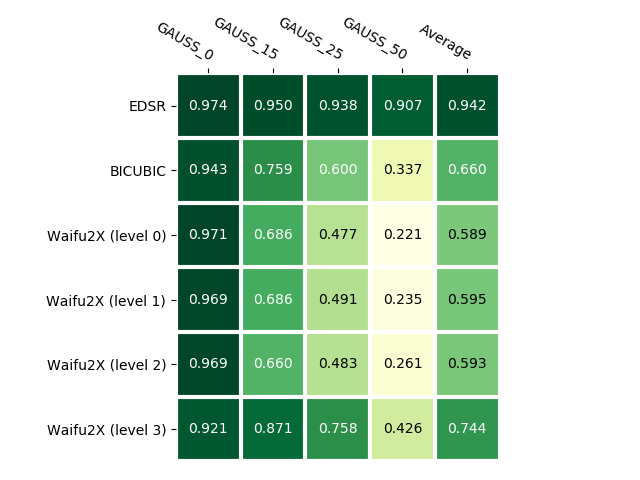
\includegraphics[width=\textwidth]{Figures/2X/Bear/SSIM_GAUSS.png}
            \caption{SSIM results with gaussian noise}
        \end{subfigure}
        \quad
        \begin{subfigure}[b]{0.475\textwidth}   
            \centering 
            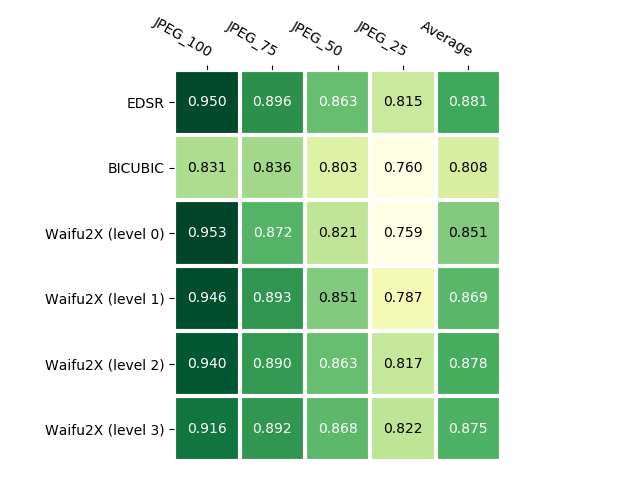
\includegraphics[width=\textwidth]{Figures/2X/Bear/SSIM_JPEG.png}
            \caption{SSIM results with JPEG noise}
        \end{subfigure}
        \caption{PSNR and SSIM results on the shown image}
    \end{figure*}
    
        \begin{figure*}
        \centering
        \begin{subfigure}[b]{0.75\textwidth}
            \centering
            \includegraphics[width=\textwidth]{Figures/2X/Catch/image.png}
            \caption{High Resolution}
        \end{subfigure}
        \vskip\baselineskip
        \begin{subfigure}[b]{0.475\textwidth}
            \centering
            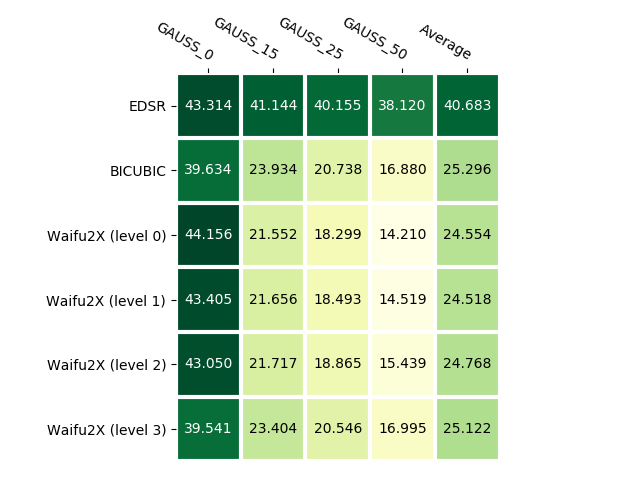
\includegraphics[width=\textwidth]{Figures/2X/Catch/PSNR_GAUSS.png}
            \caption{PSNR results with gaussian noise}
        \end{subfigure}
        \hfill
        \begin{subfigure}[b]{0.475\textwidth}  
            \centering 
            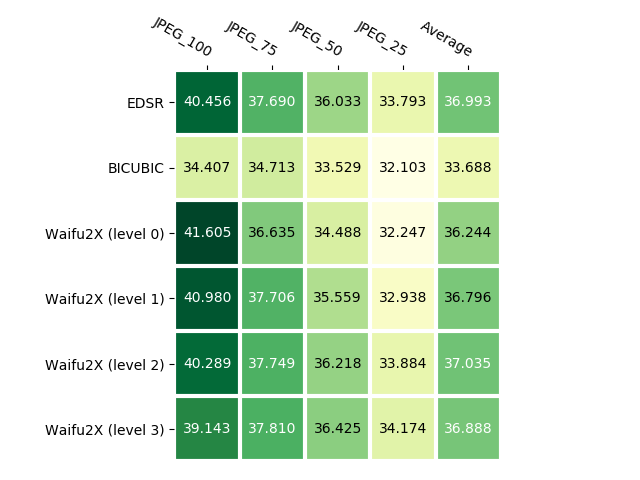
\includegraphics[width=\textwidth]{Figures/2X/Catch/PSNR_JPEG.png}
            \caption{PSNR results with JPEG noise}
        \end{subfigure}
        \vskip\baselineskip
        \begin{subfigure}[b]{0.475\textwidth}   
            \centering 
            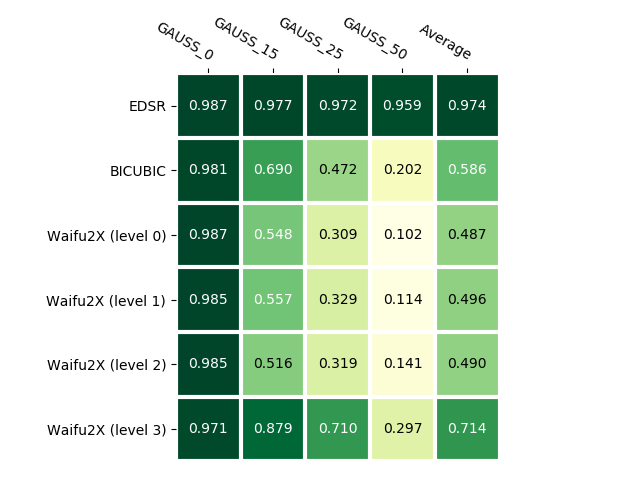
\includegraphics[width=\textwidth]{Figures/2X/Catch/SSIM_GAUSS.png}
            \caption{SSIM results with gaussian noise}
        \end{subfigure}
        \quad
        \begin{subfigure}[b]{0.475\textwidth}   
            \centering 
            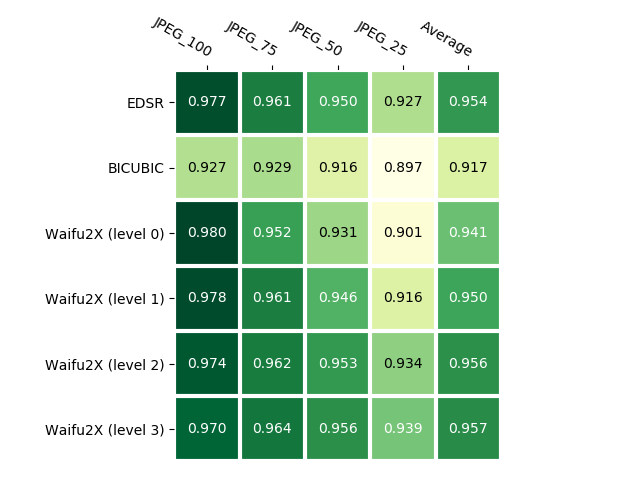
\includegraphics[width=\textwidth]{Figures/2X/Catch/SSIM_JPEG.png}
            \caption{SSIM results with JPEG noise}
        \end{subfigure}
        \caption{PSNR and SSIM results on the shown image}
    \end{figure*}
    
            \begin{figure*}
        \centering
        \begin{subfigure}[b]{0.75\textwidth}
            \centering
            \includegraphics[width=\textwidth]{Figures/2X/Coffee/image.png}
            \caption{High Resolution}
        \end{subfigure}
        \vskip\baselineskip
        \begin{subfigure}[b]{0.475\textwidth}
            \centering
            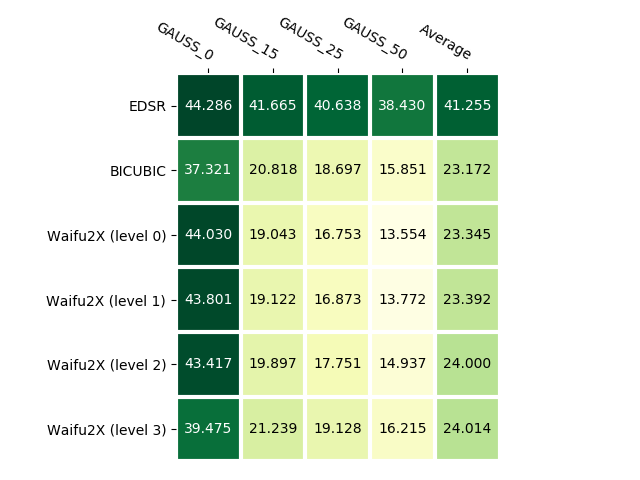
\includegraphics[width=\textwidth]{Figures/2X/Coffee/PSNR_GAUSS.png}
            \caption{PSNR results with gaussian noise}
        \end{subfigure}
        \hfill
        \begin{subfigure}[b]{0.475\textwidth}  
            \centering 
            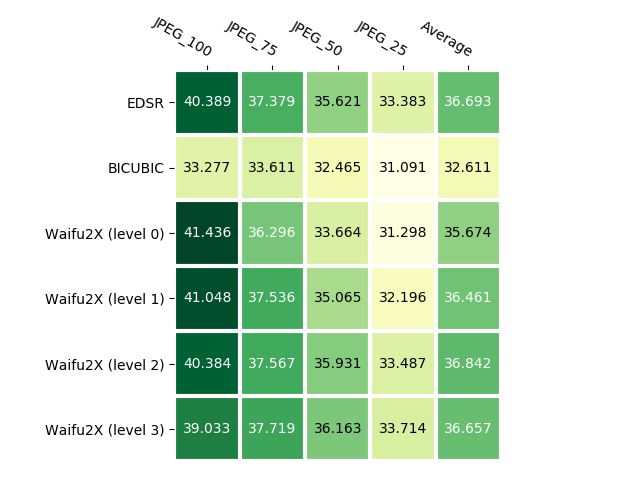
\includegraphics[width=\textwidth]{Figures/2X/Coffee/PSNR_JPEG.png}
            \caption{PSNR results with JPEG noise}
        \end{subfigure}
        \vskip\baselineskip
        \begin{subfigure}[b]{0.475\textwidth}   
            \centering 
            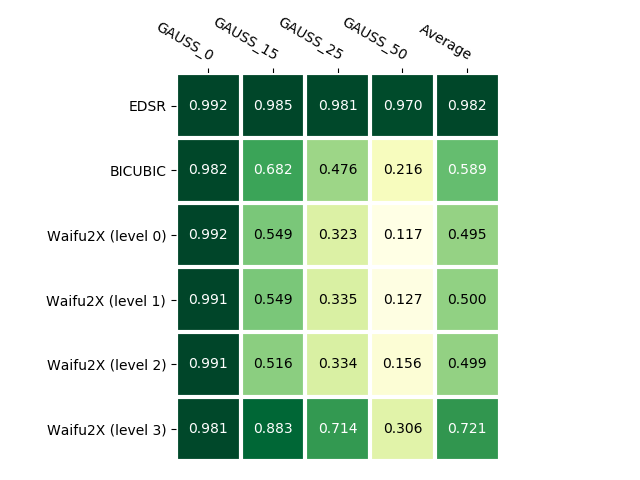
\includegraphics[width=\textwidth]{Figures/2X/Coffee/SSIM_GAUSS.png}
            \caption{SSIM results with gaussian noise}
        \end{subfigure}
        \quad
        \begin{subfigure}[b]{0.475\textwidth}   
            \centering 
            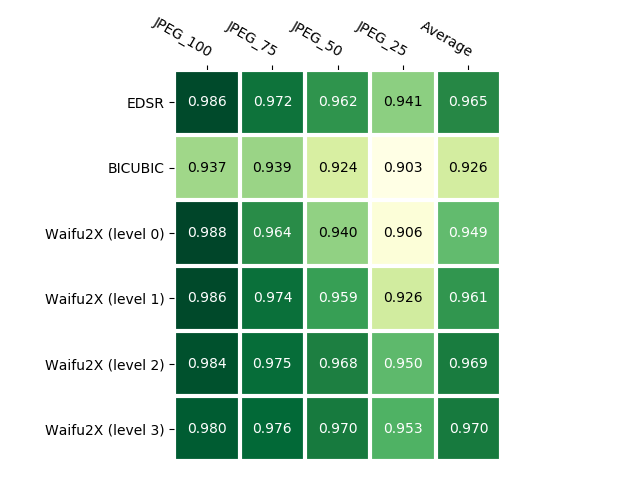
\includegraphics[width=\textwidth]{Figures/2X/Coffee/SSIM_JPEG.png}
            \caption{SSIM results with JPEG noise}
        \end{subfigure}
        \caption{PSNR and SSIM results on the shown image}
    \end{figure*}
    
            \begin{figure*}
        \centering
        \begin{subfigure}[b]{0.75\textwidth}
            \centering
            
\includegraphics[width=\textwidth]{Figures/2X/Crow/image.png}
            \caption{High Resolution}
        \end{subfigure}
        \vskip\baselineskip
        \begin{subfigure}[b]{0.475\textwidth}
            \centering
            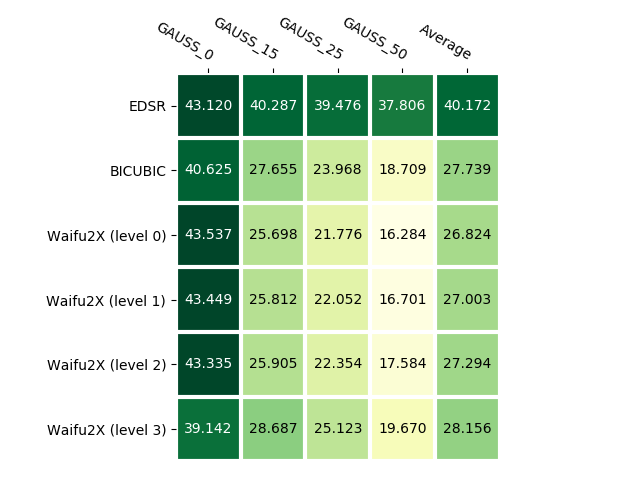
\includegraphics[width=\textwidth]{Figures/2X/Crow/PSNR_GAUSS.png}
            \caption{PSNR results with gaussian noise}
        \end{subfigure}
        \hfill
        \begin{subfigure}[b]{0.475\textwidth}  
            \centering 
            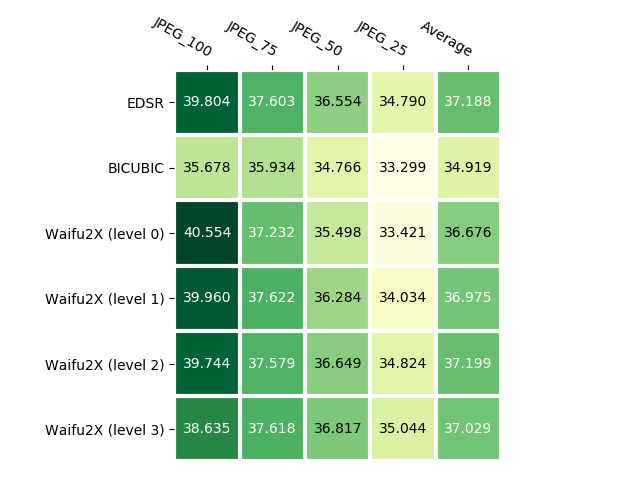
\includegraphics[width=\textwidth]{Figures/2X/Crow/PSNR_JPEG.png}
            \caption{PSNR results with JPEG noise}
        \end{subfigure}
        \vskip\baselineskip
        \begin{subfigure}[b]{0.475\textwidth}   
            \centering 
            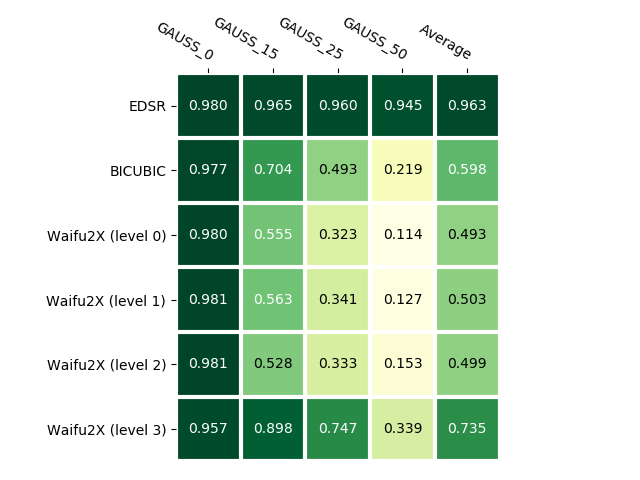
\includegraphics[width=\textwidth]{Figures/2X/Crow/SSIM_GAUSS.png}
            \caption{SSIM results with gaussian noise}
        \end{subfigure}
        \quad
        \begin{subfigure}[b]{0.475\textwidth}   
            \centering 
            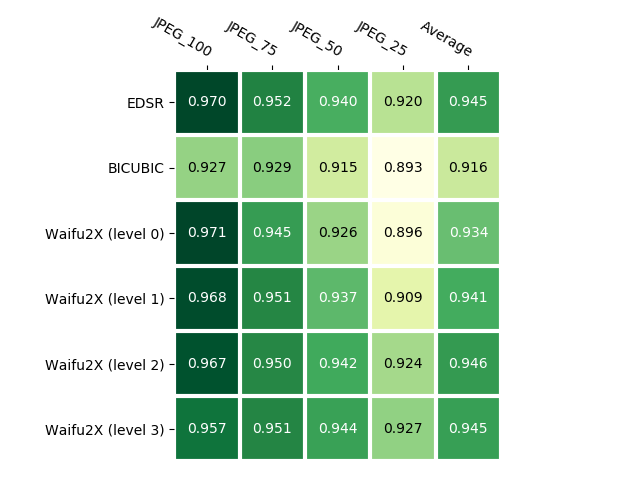
\includegraphics[width=\textwidth]{Figures/2X/Crow/SSIM_JPEG.png}
            \caption{SSIM results with JPEG noise}
        \end{subfigure}
        \caption{PSNR and SSIM results on the shown image}
    \end{figure*}
    
            \begin{figure*}
        \centering
        \begin{subfigure}[b]{0.75\textwidth}
            \centering
            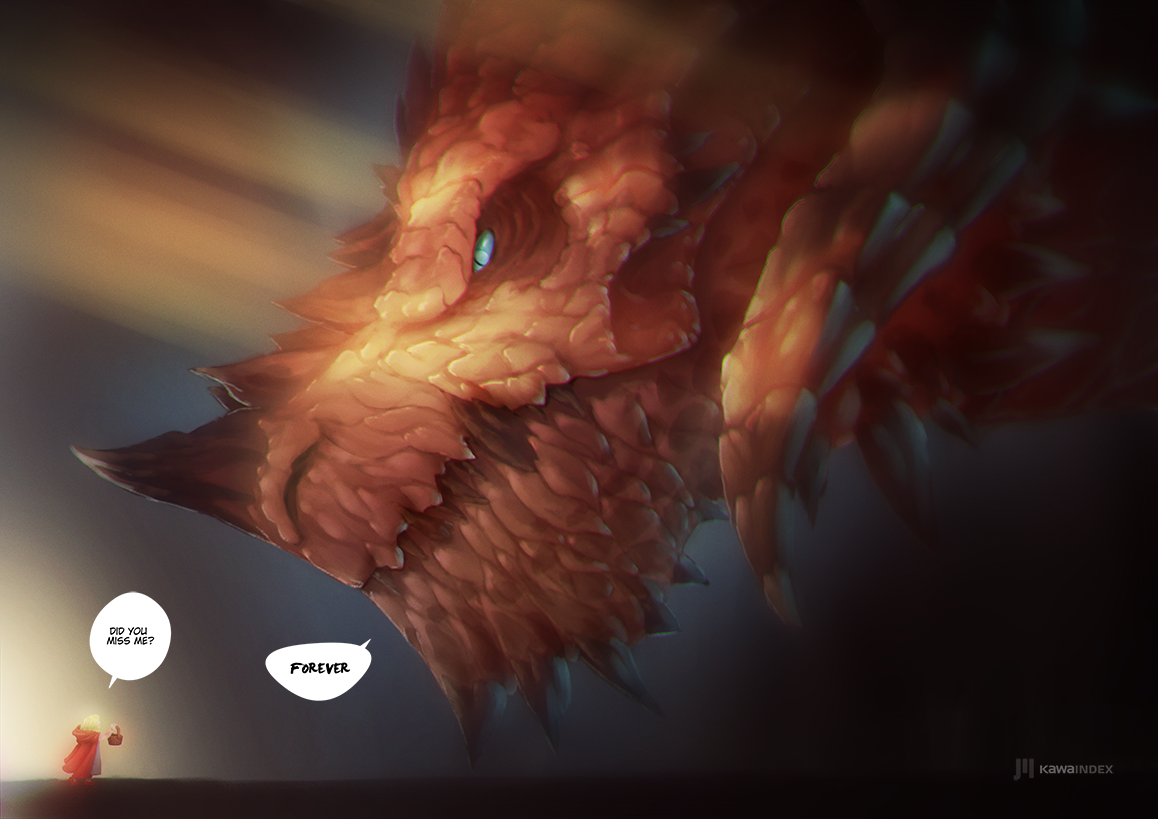
\includegraphics[width=\textwidth]{Figures/2X/Dragon/image.png}
            \caption{High Resolution}
        \end{subfigure}
        \vskip\baselineskip
        \begin{subfigure}[b]{0.475\textwidth}
            \centering
            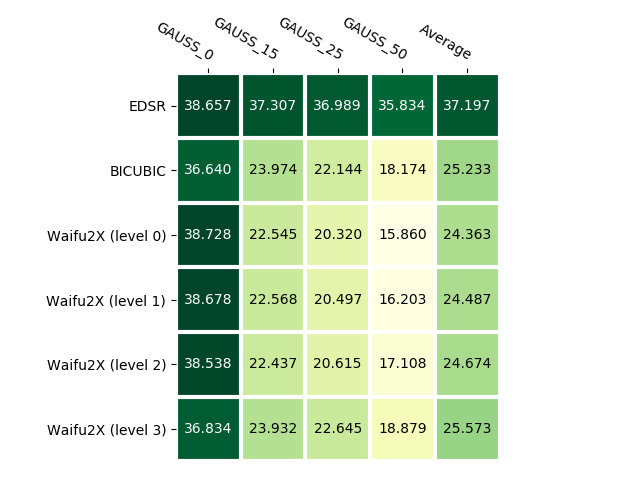
\includegraphics[width=\textwidth]{Figures/2X/Dragon/PSNR_GAUSS.png}
            \caption{PSNR results with gaussian noise}
        \end{subfigure}
        \hfill
        \begin{subfigure}[b]{0.475\textwidth}  
            \centering 
            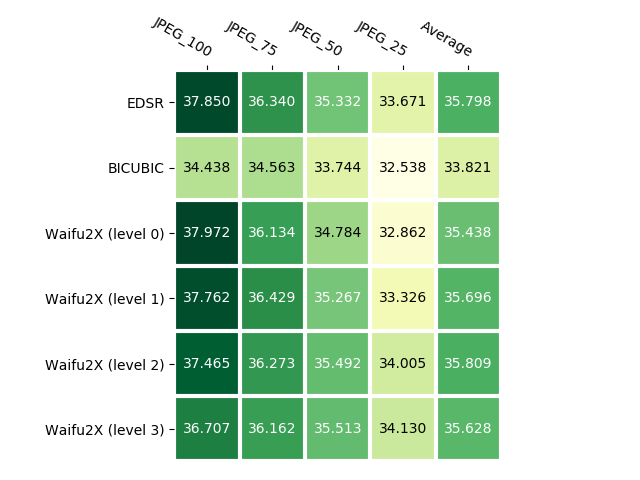
\includegraphics[width=\textwidth]{Figures/2X/Dragon/PSNR_JPEG.png}
            \caption{PSNR results with JPEG noise}
        \end{subfigure}
        \vskip\baselineskip
        \begin{subfigure}[b]{0.475\textwidth}   
            \centering 
            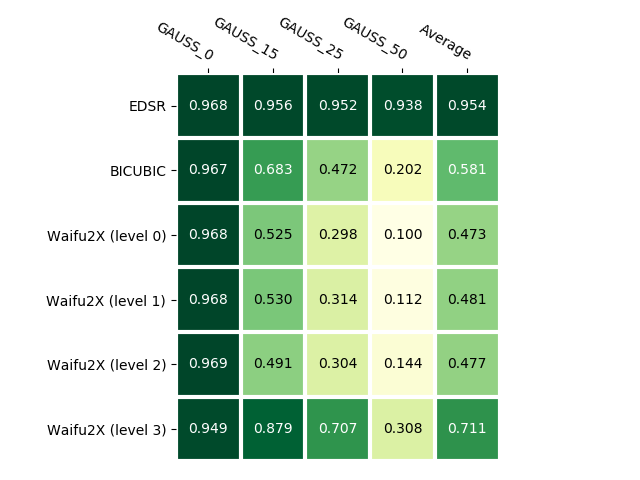
\includegraphics[width=\textwidth]{Figures/2X/Dragon/SSIM_GAUSS.png}
            \caption{SSIM results with gaussian noise}
        \end{subfigure}
        \quad
        \begin{subfigure}[b]{0.475\textwidth}   
            \centering 
            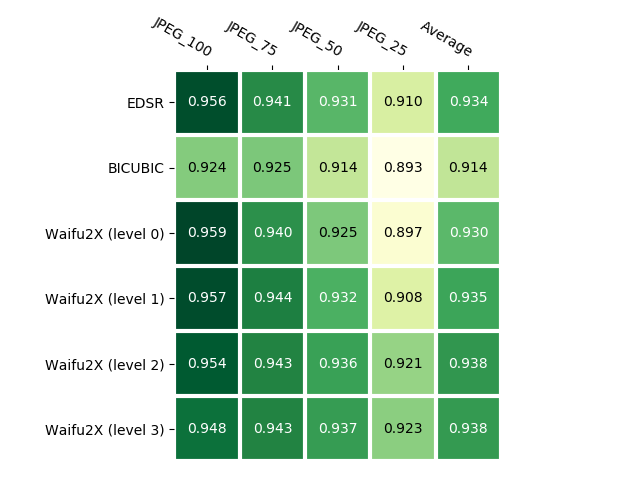
\includegraphics[width=\textwidth]{Figures/2X/Dragon/SSIM_JPEG.png}
            \caption{SSIM results with JPEG noise}
        \end{subfigure}
        \caption{PSNR and SSIM results on the shown image}
    \end{figure*}